\chapter{Nestor3: maintain a fairway }
%
%****************************************************
% - Purpose & Problem description:
%     These first two parts give reader short details about the test case,
%     the physical phenomena involved and specify how the numerical solution will be validated
\section{Purpose (Dig\_by\_criterion)}
%----------------------------------------------------
Example for Nestor:\\
dredging in case a depth criterion is violated and dumping of the dredged material.\\
\\
Details about:
\begin{itemize}
\item{\texttt{ActionType = Dig\_by\_criterion}}
\end{itemize}
%****************************************************
\section{Description of the problem}
%----------------------------------------------------
This example performs the automated maintenance of a fairway to predict the expected dredging demand.\\
At regular time intervals (\,\texttt{TimeRepeat}\,) (fig.\,\ref{E3timeschema}) Nestor tests within the
fairway polygon for each node if the depth criterion (\,\texttt{CritDepth}\,) is violated.
In case of violation the node will be dredged step-by-step with a specified rate (\,\texttt{DigRate}\,)
to a specified depth (\,\texttt{DigDepth}\,) and the dredged volume will be recorded in the listing file.\\
\\
\\
\begin{figure} [H]
 \centering
% 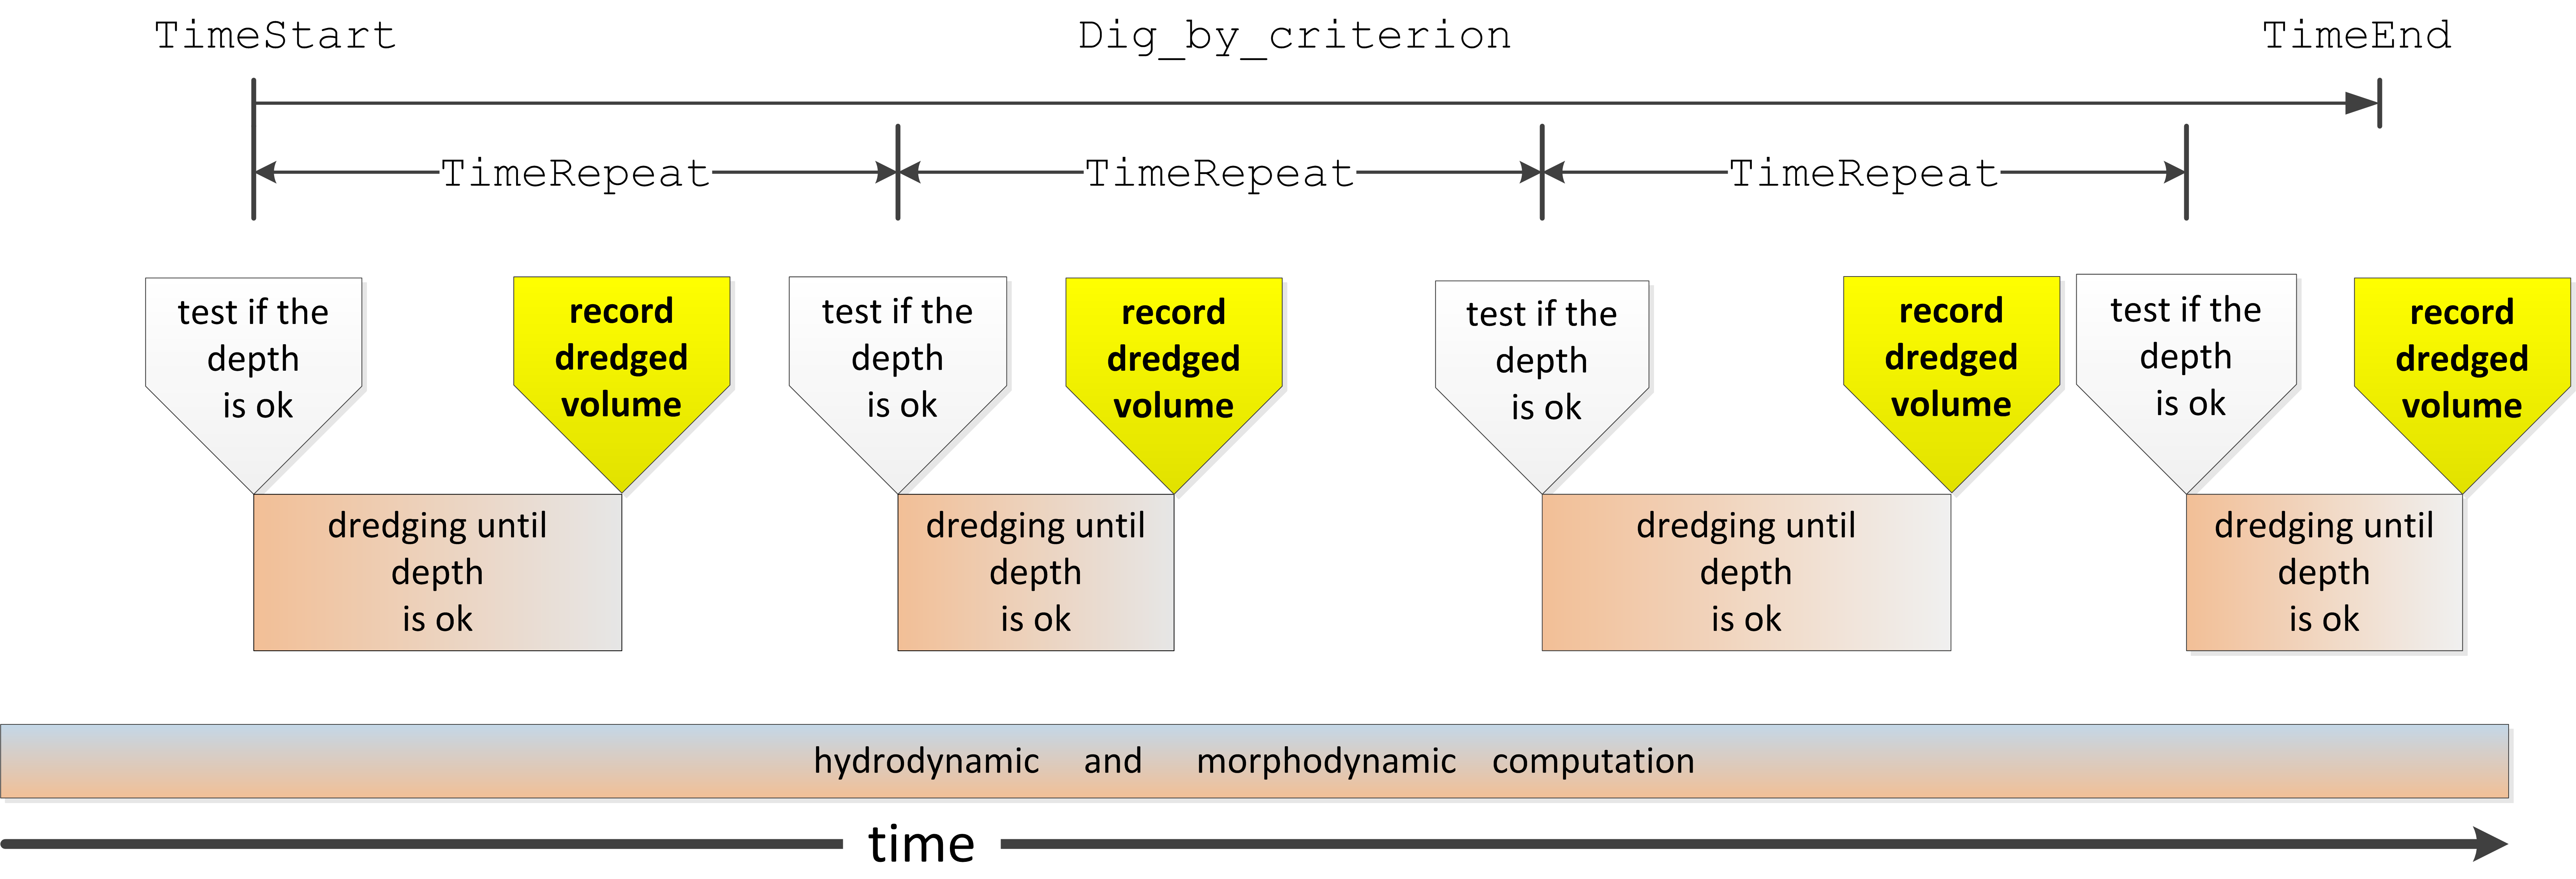
\includegraphics[scale=3.25]{img/zeitlAblaufSchema_DigByCrit.png}
 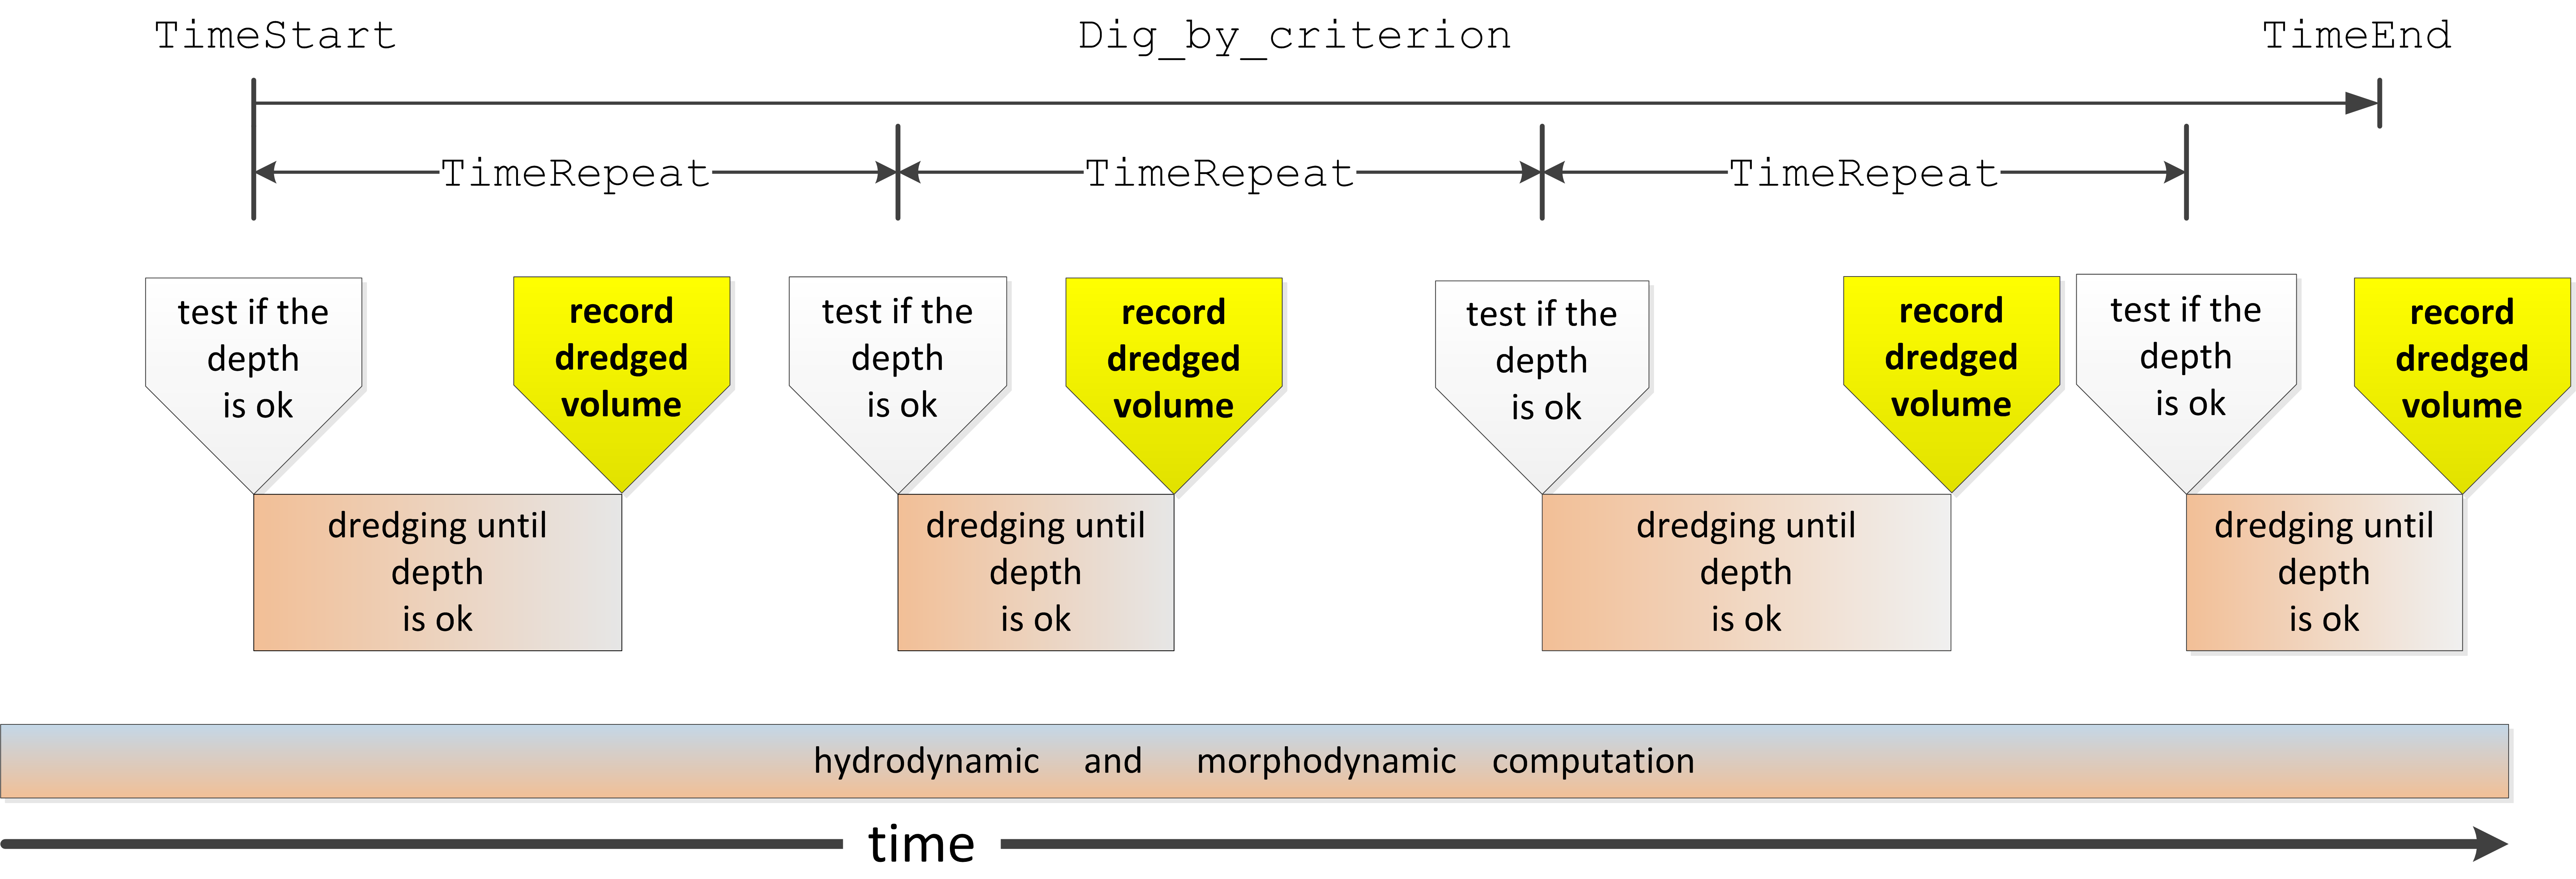
\includegraphics[width=1.0\linewidth]{img/zeitlAblaufSchema_DigByCrit.png}
 \caption{General operating schedule for dredging by criterion}\label{E3timeschema}
\end{figure}



\newpage
The node depth is defined as elevation of the reference level minus elevation of the node (fig.\,\ref{E3schema}).
\begin{figure} [H]
\centering
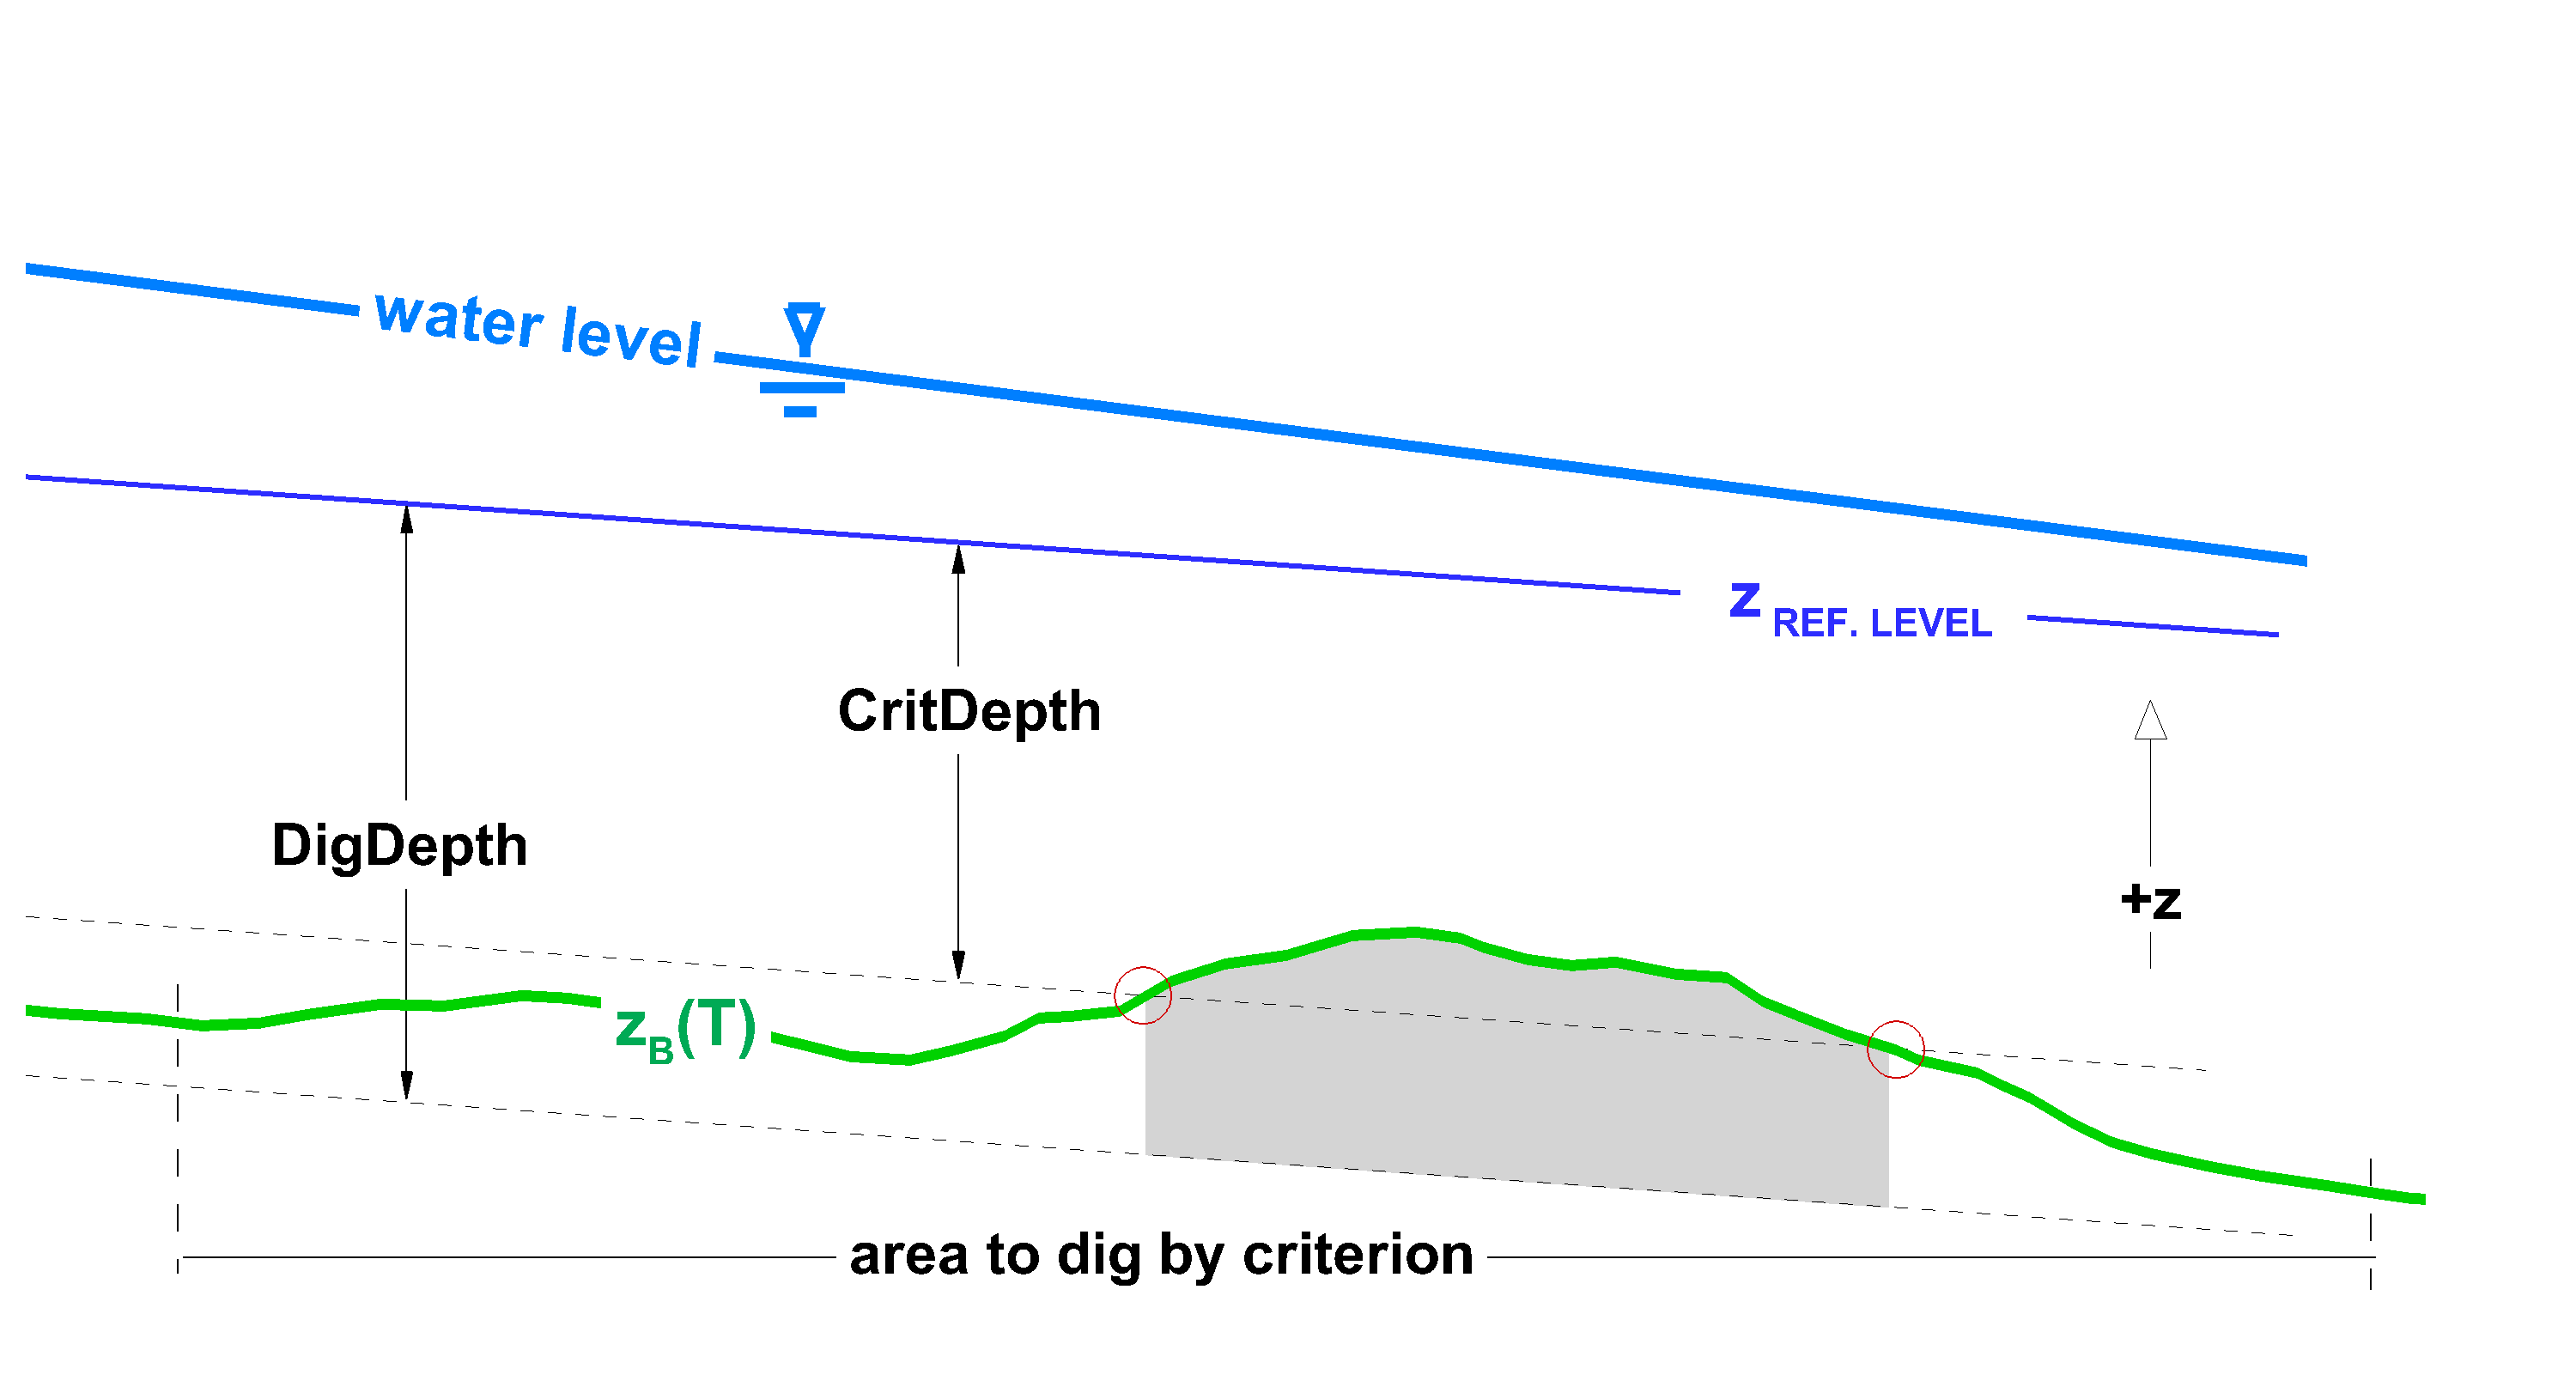
\includegraphics[scale=0.12]{img/critDig_schematicDiagram.png}
\caption{Schematic diagram of dredging by criterion}\label{E3schema}
\end{figure}

Excerpt from the action file where the Action is defined:
\\ \hspace*{3mm} \texttt{\small{/================================================================}}
\\ \hspace*{3mm} \texttt{\small{ACTION}}
\\ \hspace*{3mm} \texttt{\small{~~ActionType~~~~~~=~~Dig\_by\_criterion}}
\\ \hspace*{3mm} \texttt{\small{~~FieldDig~~~~~~~~=~~100\_Fairway}}
\\ \hspace*{3mm} \texttt{\small{~~ReferenceLevel~~=~~SECTIONS}}
\\ \hspace*{3mm} \texttt{\small{~~TimeStart~~~~~~~=~~2000.01.01-23:00:00~~/~[yyyy.mm.dd-hh:mm:ss]}}
\\ \hspace*{3mm} \texttt{\small{~~TimeRepeat~~~~~~=~~860000.0~~~~~~~~~~~~~/~[~s~] 10 days}}
\\ \hspace*{3mm} \texttt{\small{~~TimeEnd~~~~~~~~~=~~2000.01.12-23:59:59~~/~[yyyy.mm.dd-hh:mm:ss]}}
\\ \hspace*{3mm} \texttt{\small{~~DigRate~~~~~~~~~=~~~0.001~~~~~~~~~~~~~~~/~[~m/s~]}}
\\ \hspace*{3mm} \texttt{\small{~~DigDepth~~~~~~~~=~~10.00~~~~~~~~~~~~~~~~/~[~m~]}}
\\ \hspace*{3mm} \texttt{\small{~~CritDepth~~~~~~~=~~10.00~~~~~~~~~~~~~~~~/~[~m~]}}
\\ \hspace*{3mm} \texttt{\small{~~MinVolume~~~~~~~=~~~0.0~~~~~~~~~~~~~~~~~/~[~m\textasciicircum3~]}}
\\ \hspace*{3mm} \texttt{\small{~~MinVolumeRadius~=~~~3.5~~~~~~~~~~~~~~~~~/~[~m~]}}
\\ \hspace*{3mm}
\\ \hspace*{3mm} \texttt{\small{~~FieldDump~~~~~~~=~~200\_DumpArea}}
\\ \hspace*{3mm} \texttt{\small{~~DumpRate~~~~~~~~=~~~0.001~~~~~~~~~~~~~~~/~[~m/s~]}}
\\ \hspace*{3mm} \texttt{\small{~~DumpPlanar~~~~~~=~~FALSE}}
\\ \hspace*{3mm} \texttt{\small{ENDACTION}}
\\ \hspace*{3mm} \texttt{\small{/================================================================}}\\
\\
The reference level is defined by 17 sections (see black lines in fig.\,\ref{E3grid}) which are defined in file \texttt{\_DigRefLev.dat}.
Because \texttt{~FieldDump~} is used, the dredged material is transferred (dumped) to the dumping area.
The fairway and the dumping area (fig.\,\ref{E3grid}) are defined by polygons which are defined in file \texttt{\_DigPolys.dat}.\\
About \texttt{~MinVolume~} and \texttt{~MinVolumeRadius }:~~~
In reality, it may still be acceptable for the fairway to have small shallows.
Normally dredging will not be induced until the shallow becomes as serious problem
or has grown to such a volume where it is worthwhile to call the dredge.
To mirror this approach there are two keywords used to determine if Judge Dredd needs to pay a visit.
In case a node (e.g. node-A) violates the depht criterion, Nestor adds up the derdge volume of the nodes in the neighborhood.
If the sum exceeds the value of \texttt{~MinVolume~} node-A will be dredged.
The size of the neighborhood is sepcified by the keyword \texttt{~MinVolumeRadius~}.
\\

%****************************************************
% - Physical parameters:
%     This part specifies the geometry, details all the physical parameters
%     used to describe both porous media (soil model in particularly) and
%     solute characteristics (dispersion/diffusion coefficients, soil <=> pollutant interactions...)
\subsection{Physical parameters}
%----------------------------------------------------
The simulation is set up with 1 grain class.
The rigid bed is 3.0\,m below the initial (flat) bottom.
The Meyer-Peter Mueller (MPM) transport formula is used with default settings.
Thus all bottom changes are a result of sediment transport processes and fairway maintenance (dredging and dumping).

%****************************************************
% - Geometry and Mesh:
%     This part describes the mesh used in the computation
\subsection{Geometry and Mesh}
%----------------------------------------------------
A 3.3\,km long flume with two 180\,$^\circ$ bends has been chosen as test geometry.
The width of the flume is 200\,m (fig.\,\ref{E3grid}).\\
The mesh consists of 1614 nodes and 2948 elements.

\begin{figure} [!h]
\centering
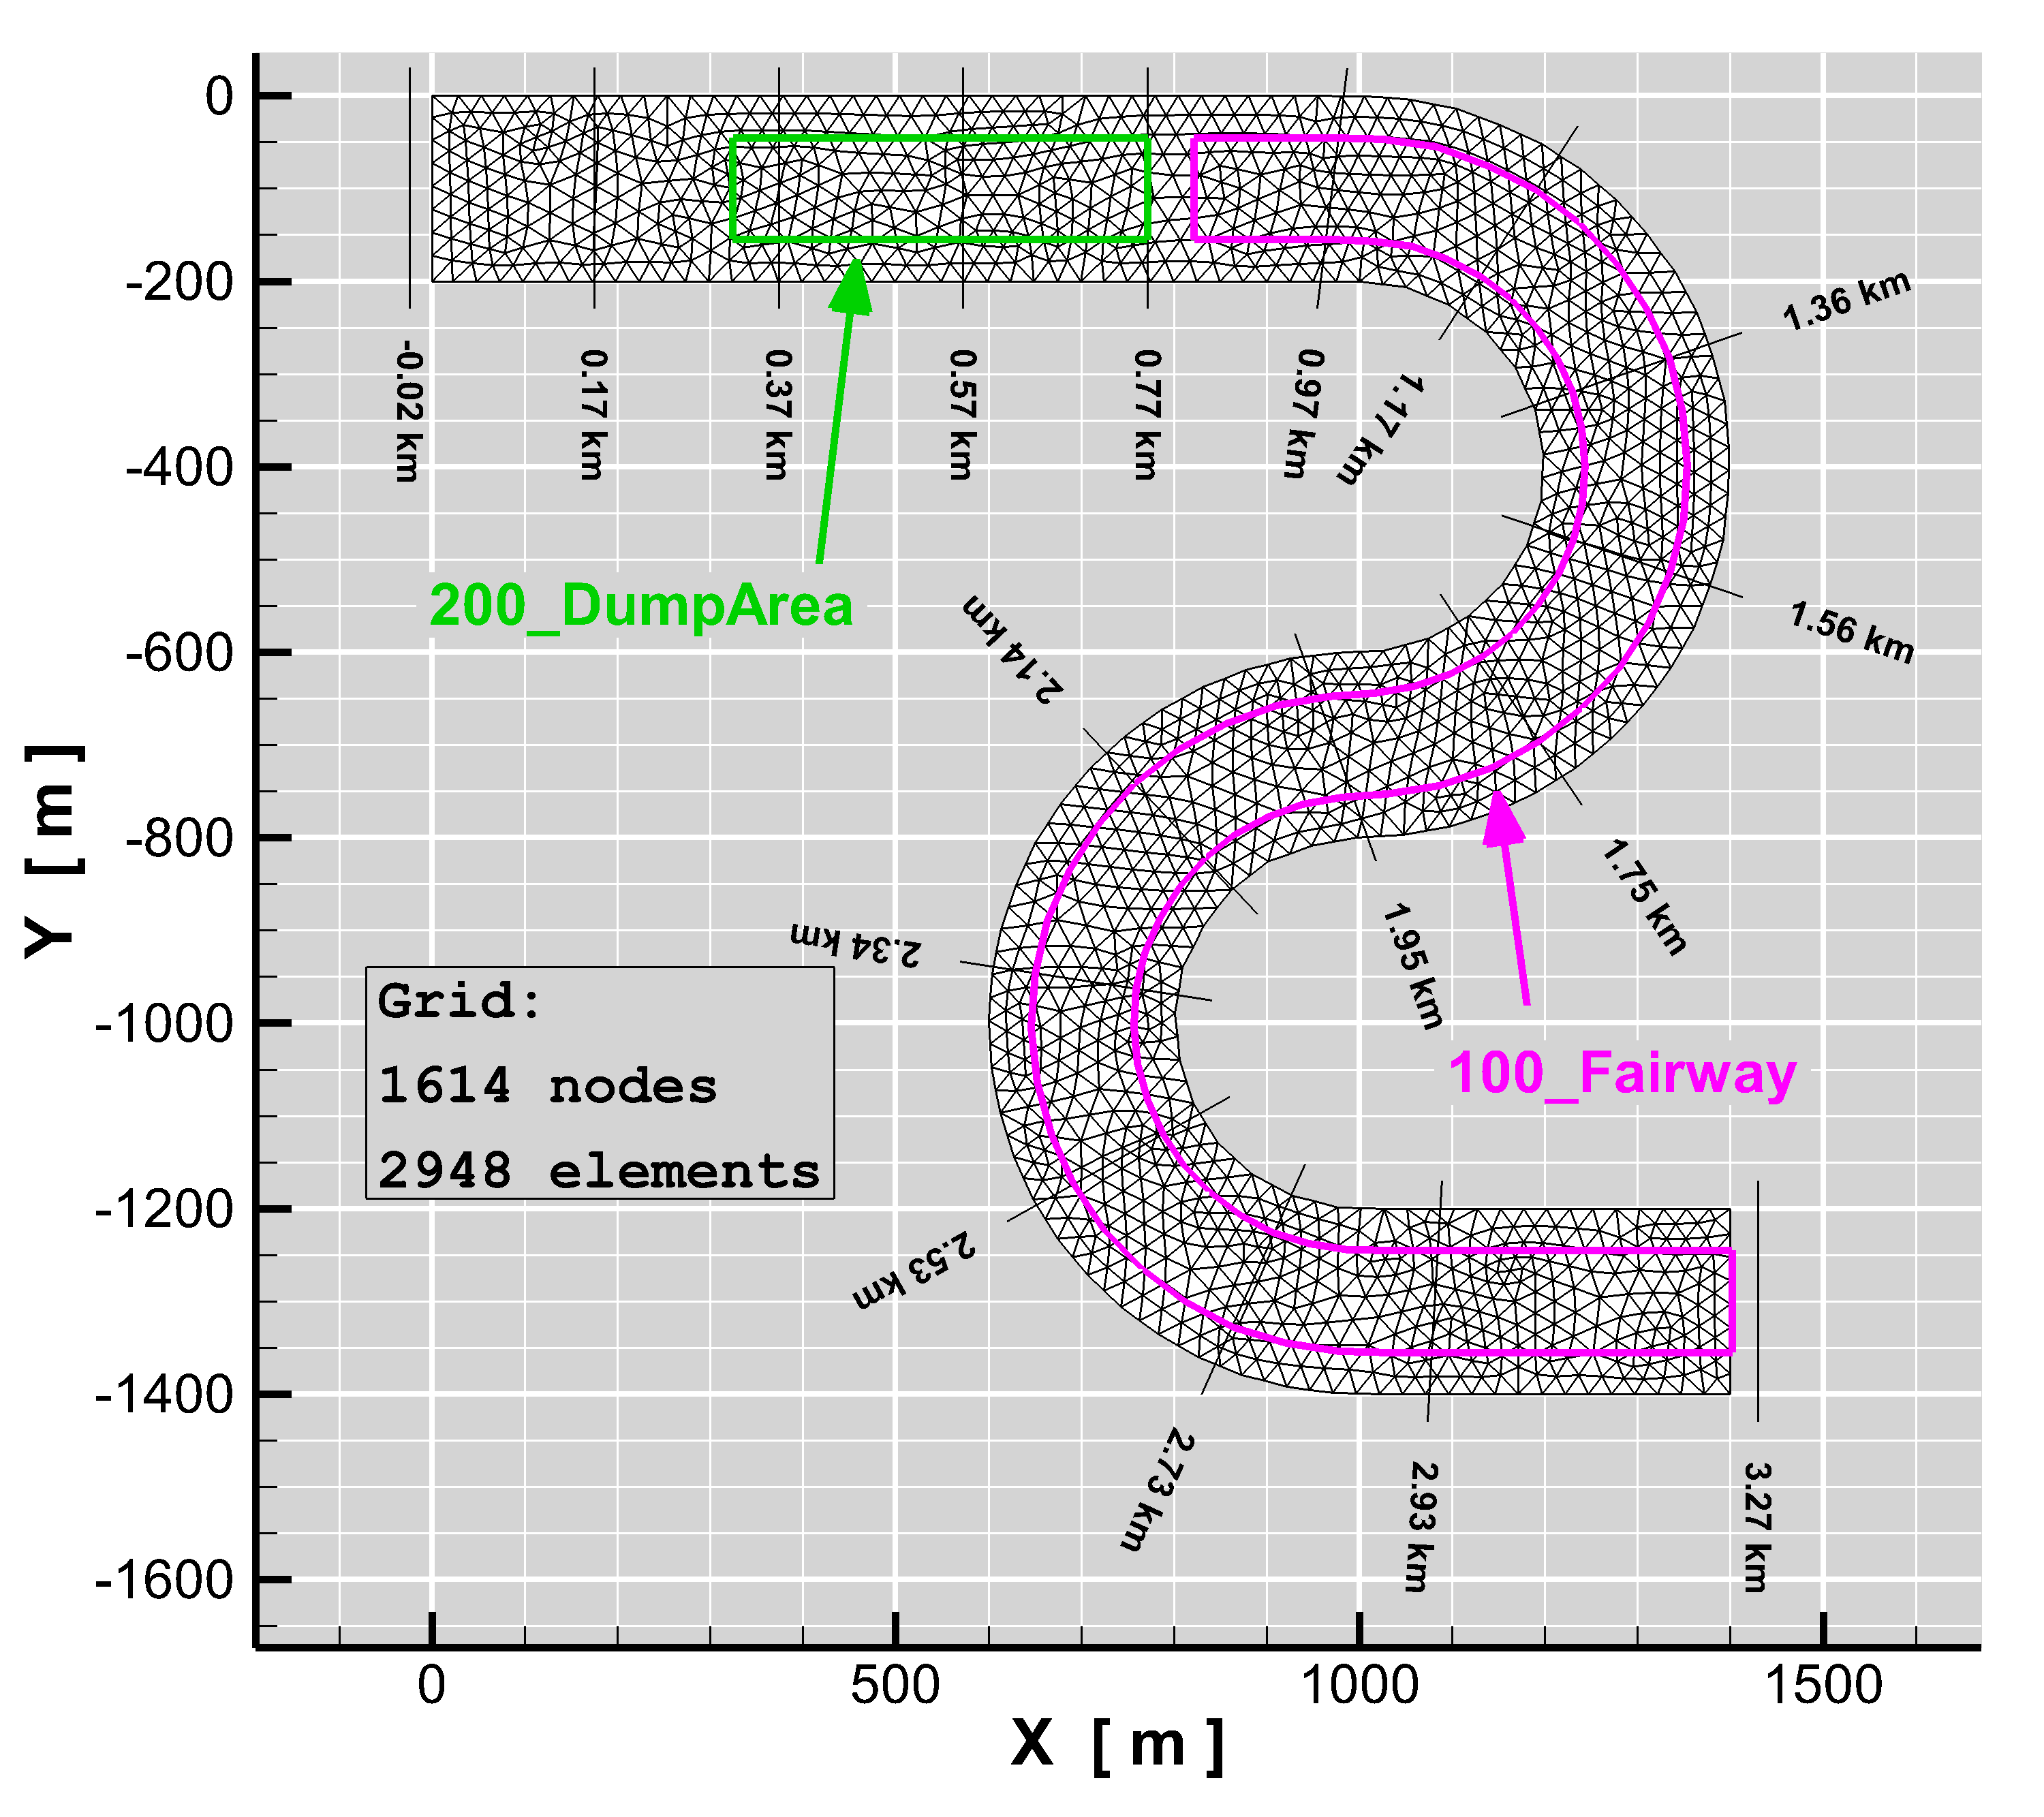
\includegraphics[scale=0.14]{img/critDig_grid_Polys_2D.png}
\caption{Geometry of the test flume with two bends and two polygons (fairway, dump area) and sections to define the reference level}\label{E3grid}
\end{figure}

%****************************************************
% - Initial and boundary conditions:
%     This part details both initial and boundary conditions used to simulate the case
\subsection{Initial and Boundary Conditions}
%----------------------------------------------------
Steady state boundary conditions:\\
\hspace*{3mm} - Discharge at the inlet = 1000\,m$^3$/s\\
\hspace*{3mm} - Water level at the outlet = 2.2\,m\\
\hspace*{3mm} - Sedimentological equilibrium at the inlet (zF is constant, QS is calculated)\\
\\
Initial hydraulic conditions:\\
\hspace*{3mm} - Fully developed flow from a previous simulation is used as initial hydraulic condition.\\
\\
Initial morphological conditions:\\
\hspace*{3mm} - The bottom shape and\\
\hspace*{3mm} - the ground composition is resumed from a previous simulation.\\
\\
The simulation period is 1200000.0\,s (13.88 days) with a time step of 4\,s.


%****************************************************
% - Results:
%     We comment in this part the numerical results against the reference ones,
%     giving understanding keys and making assumptions when necessary.
\section{Results} \label{sec:E3Result}
%----------------------------------------------------
To find some information about when the action was active and what was going on,
search in the telemac listing file for lines with \texttt{"\textbf{?>}"} at the beginning.\\
\\
Excerpt from the telemac listing with information about the action status:\\
\\~\hspace*{3mm}~\texttt{\small{~:~}}
\\~\hspace*{3mm}~\texttt{\small{~?>~info:========================================================+}}
\\~\hspace*{3mm}~\texttt{\small{~?>~info:~~~~~~~~~~~~~~~~~~~~~~~~~~~~~~~~~~~~~~~~~~~~~~~~~~~~~~~~|}}
\\~\hspace*{3mm}~\texttt{\small{~?>~info:~~~~~~~~~~~~NESTOR~~~~~~~~~~~~~~~~~~~~~~~~~~~~~~~~~~~~~~|}}
\\~\hspace*{3mm}~\texttt{\small{~?>~~~~~~~~~~~~~~~~~~~~~~~~~~~~~~~~~~~~~~~~~~~~~~~~~~~~~~~~~~~~~~~}}
\\~\hspace*{3mm}~\texttt{\small{~?>~~~~~~~~~~~~~~~~~~~:~~~~~~~~~~~~~~~~~~~~~~~~~~~~~~~~~~~~~~~~~~~~}}
\\~\hspace*{3mm}~\texttt{\small{~?>~~~~~~~~~~~~~~~~~~~:~~~~~~~~~~~~~~~~~~~~~~~~~~~~~~~~~~~~~~~~~~~~}}
\\~\hspace*{3mm}~\texttt{\small{~?>~info:========================================================+}}
\\~\hspace*{3mm}~\texttt{\small{~:~}}\\
\\
\\
\\
%\newpage
When a node reaches the target depth a line with information about:\\
\hspace*{3mm} - the volume of dredged material\\
\hspace*{3mm} - location of the node\\
\hspace*{3mm} - time when the dredging did start and ended \\
will be written to the listing file. These lines are marked with the label \texttt{~XdigX~}.\\
(see chpt.\,\ref{sssec:E1NodeInfo}\,/\,page\,\pageref{txt:E1XdigX})
 \label{txt:E3XdigX}\\
\\
Figure \ref{result12} shows the bottom evolution after 0\,h and 1\,h. The evolution after 0\,d is from a previous computation file.
The evolution after 1\,d is driven by the first maintenance of the fairway and sediment transport.
The digging and dumping were executed between 0\,d and 1\,d.
The fairway was dredged to the \texttt{DigDepth} and the dredged material was dumped to the dumping area
defined by the polygon \texttt{200\_DumpArea}.\\
Figure \ref{result34} and \ref{result56} shows the bottom evolution due to sediment transport processes after 3\,d, 7\,d and 10\,d.
No digging and dumping actions were defined in this time period. Between 10\,d and 11\,d the second maintenance was executed.
Again the fairway was dredged to the \texttt{DigDepth} and the dredged material was dumped to the dumping area, which
leaded again to a higher bottom evolution.

Figure \ref{result78} shows the bottom evolution  12\,d and 13.5\,d due to sediment transport processes after the
second maintenance of the fairway.

% Here is an example of how to include the graph generated by validateTELEMAC.py
% They should be in test_case/img
\begin{figure} [!h]
\centering
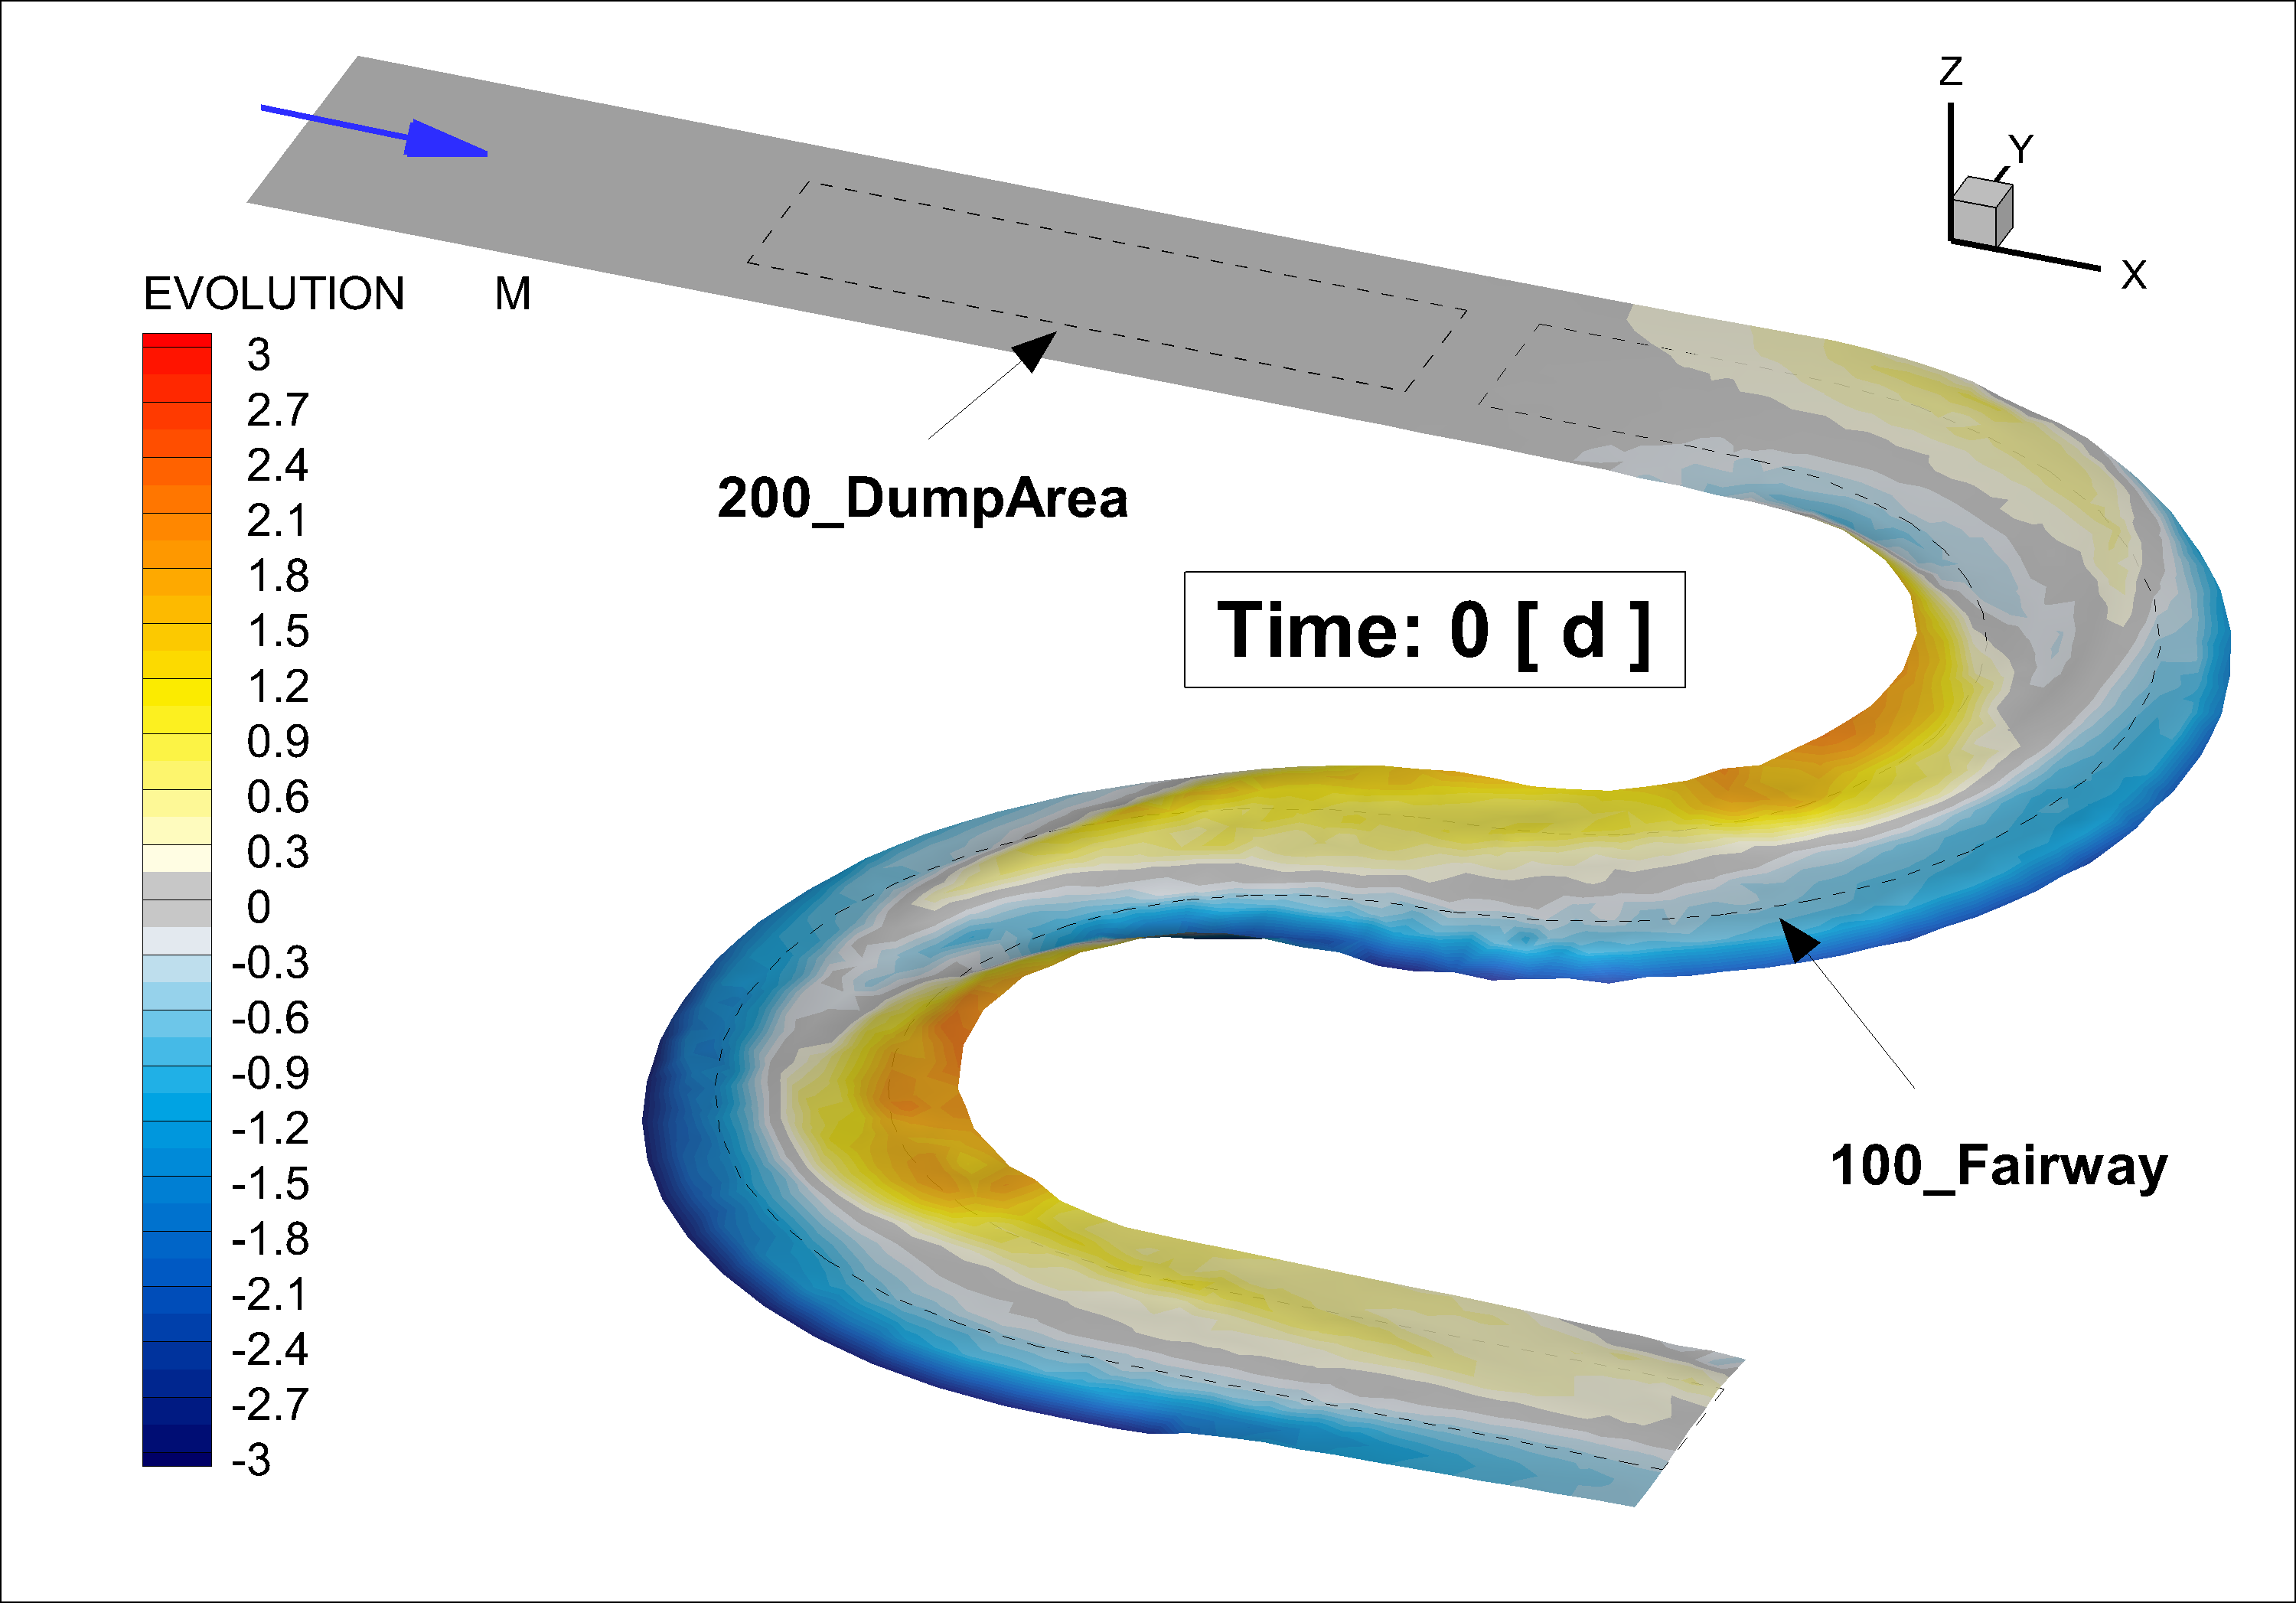
\includegraphics[scale=0.14]{img/critDig_Poly_00p0d.png}
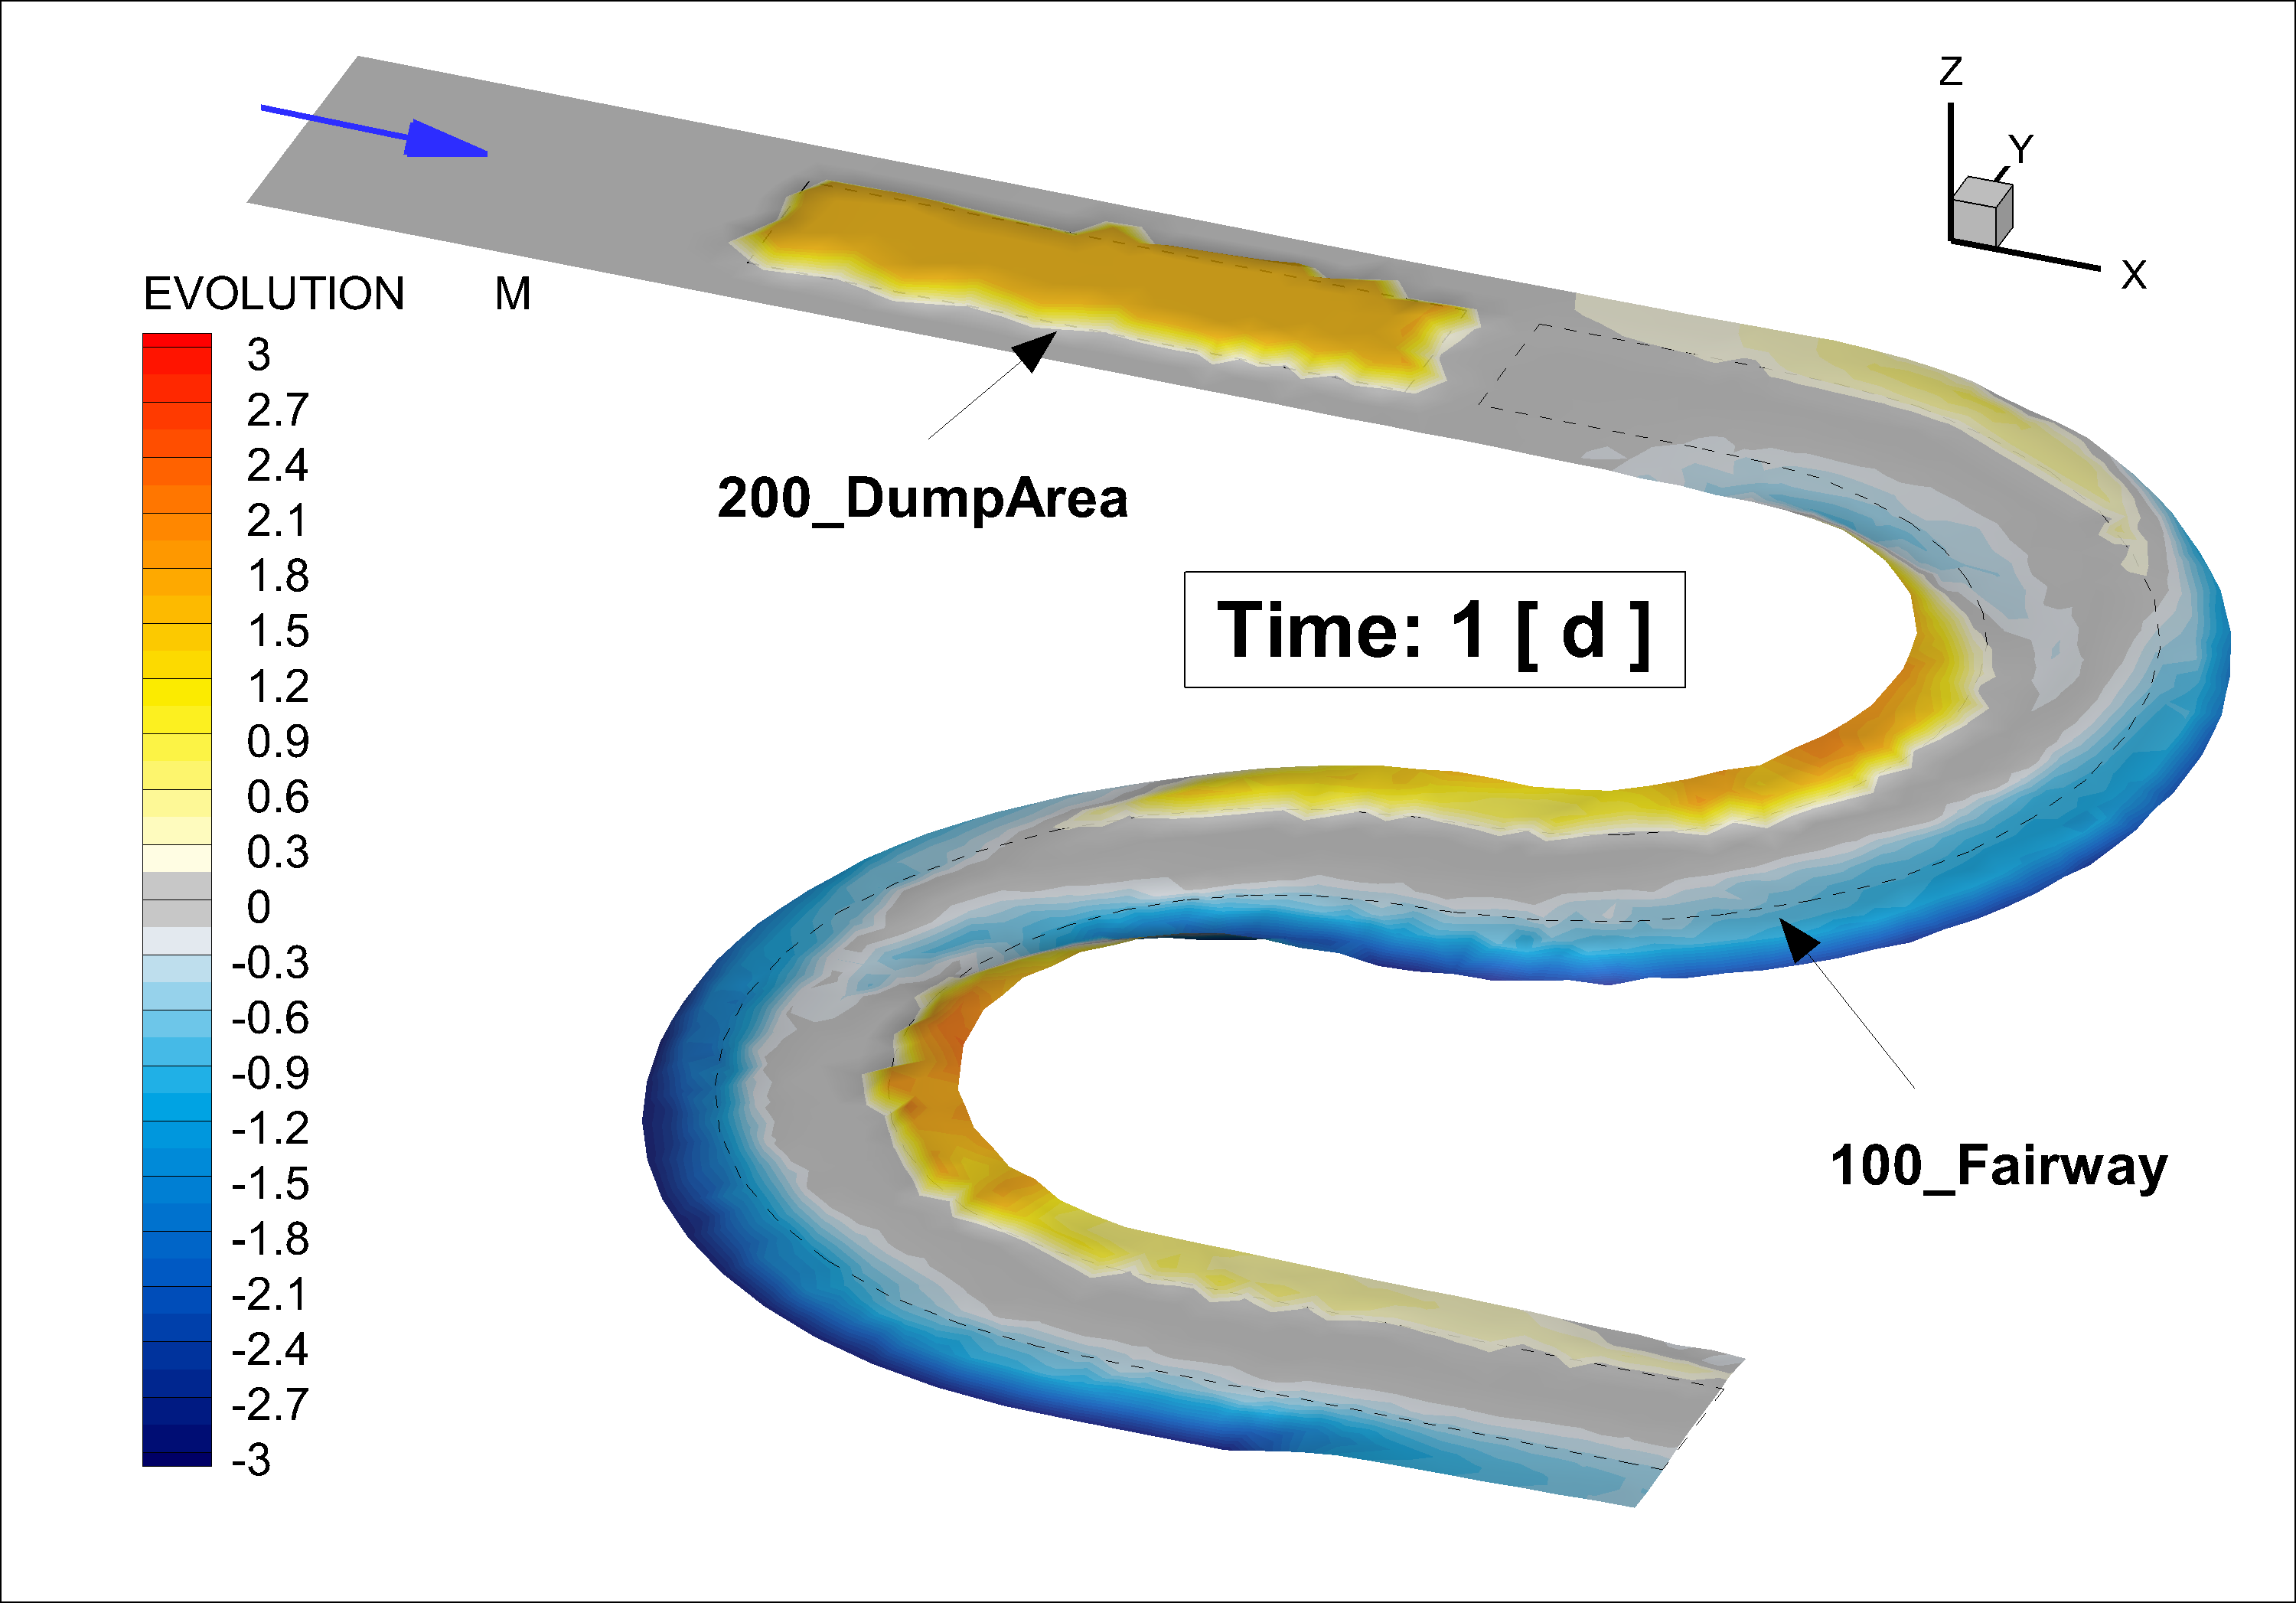
\includegraphics[scale=0.14]{img/critDig_Poly_01p0d.png}
\caption{Simulated evolution over the time.}\label{result12}
\end{figure}

\begin{figure} [!h]
\centering
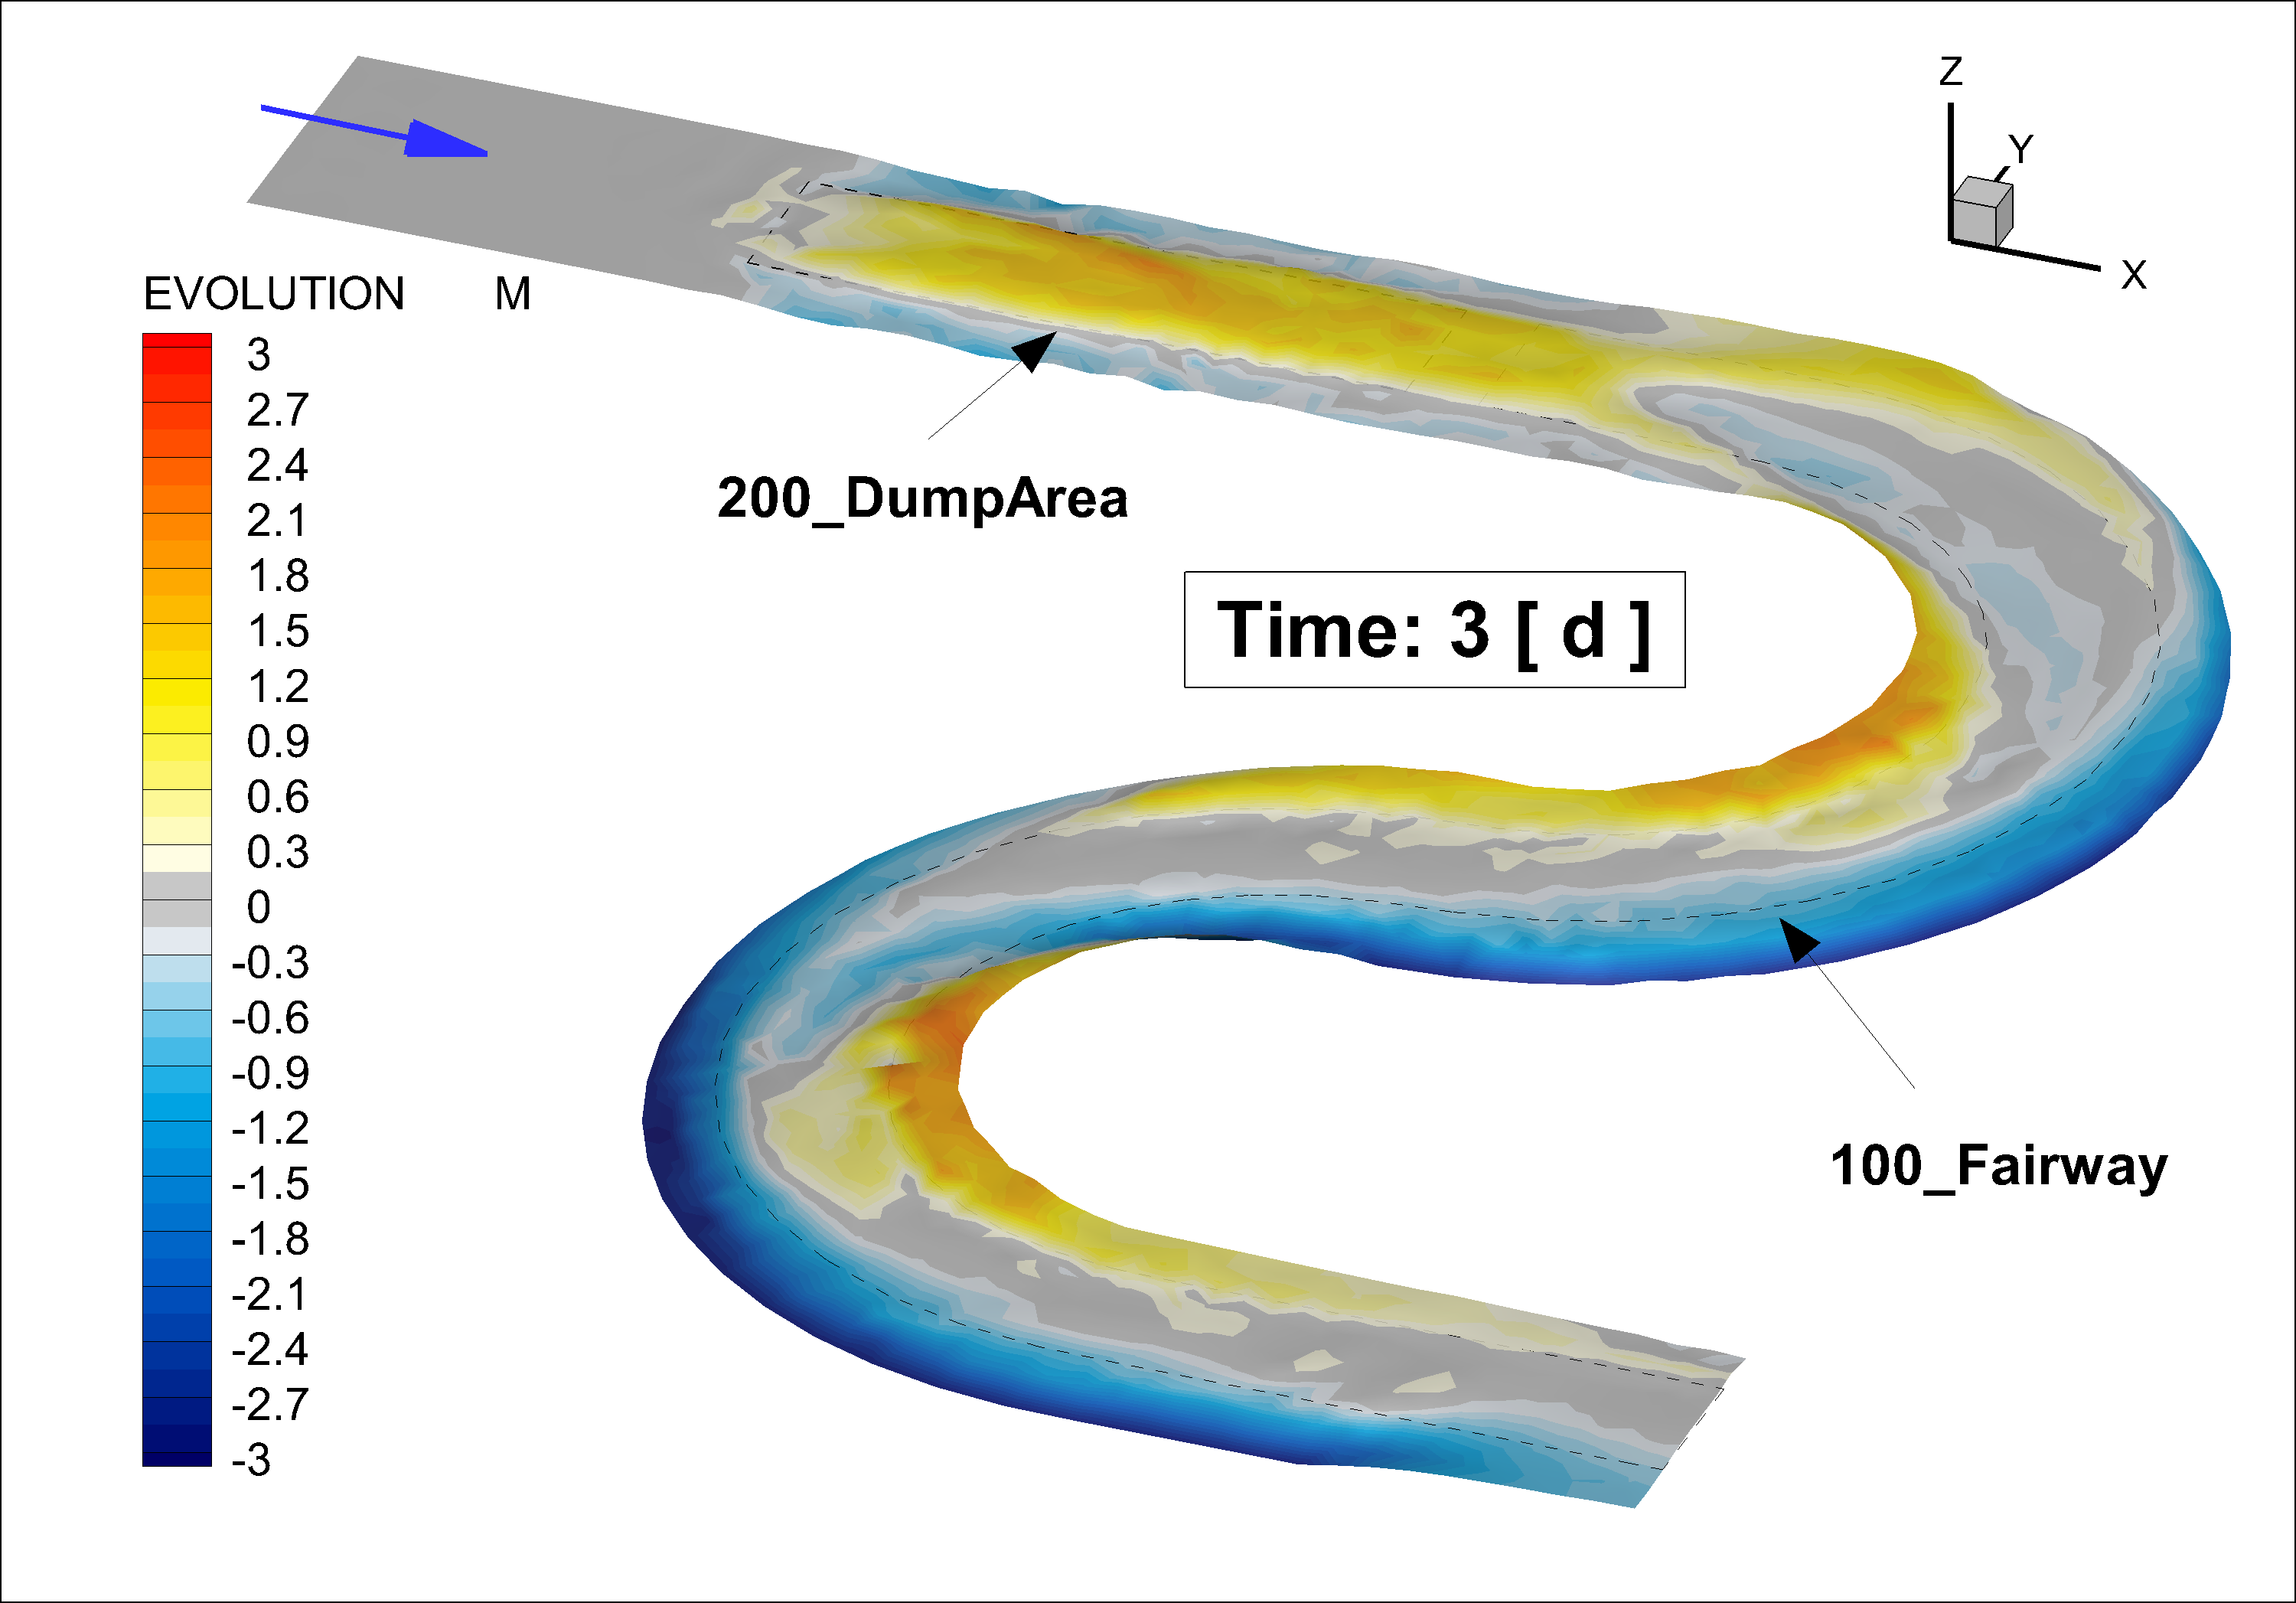
\includegraphics[scale=0.14]{img/critDig_Poly_03p0d.png}
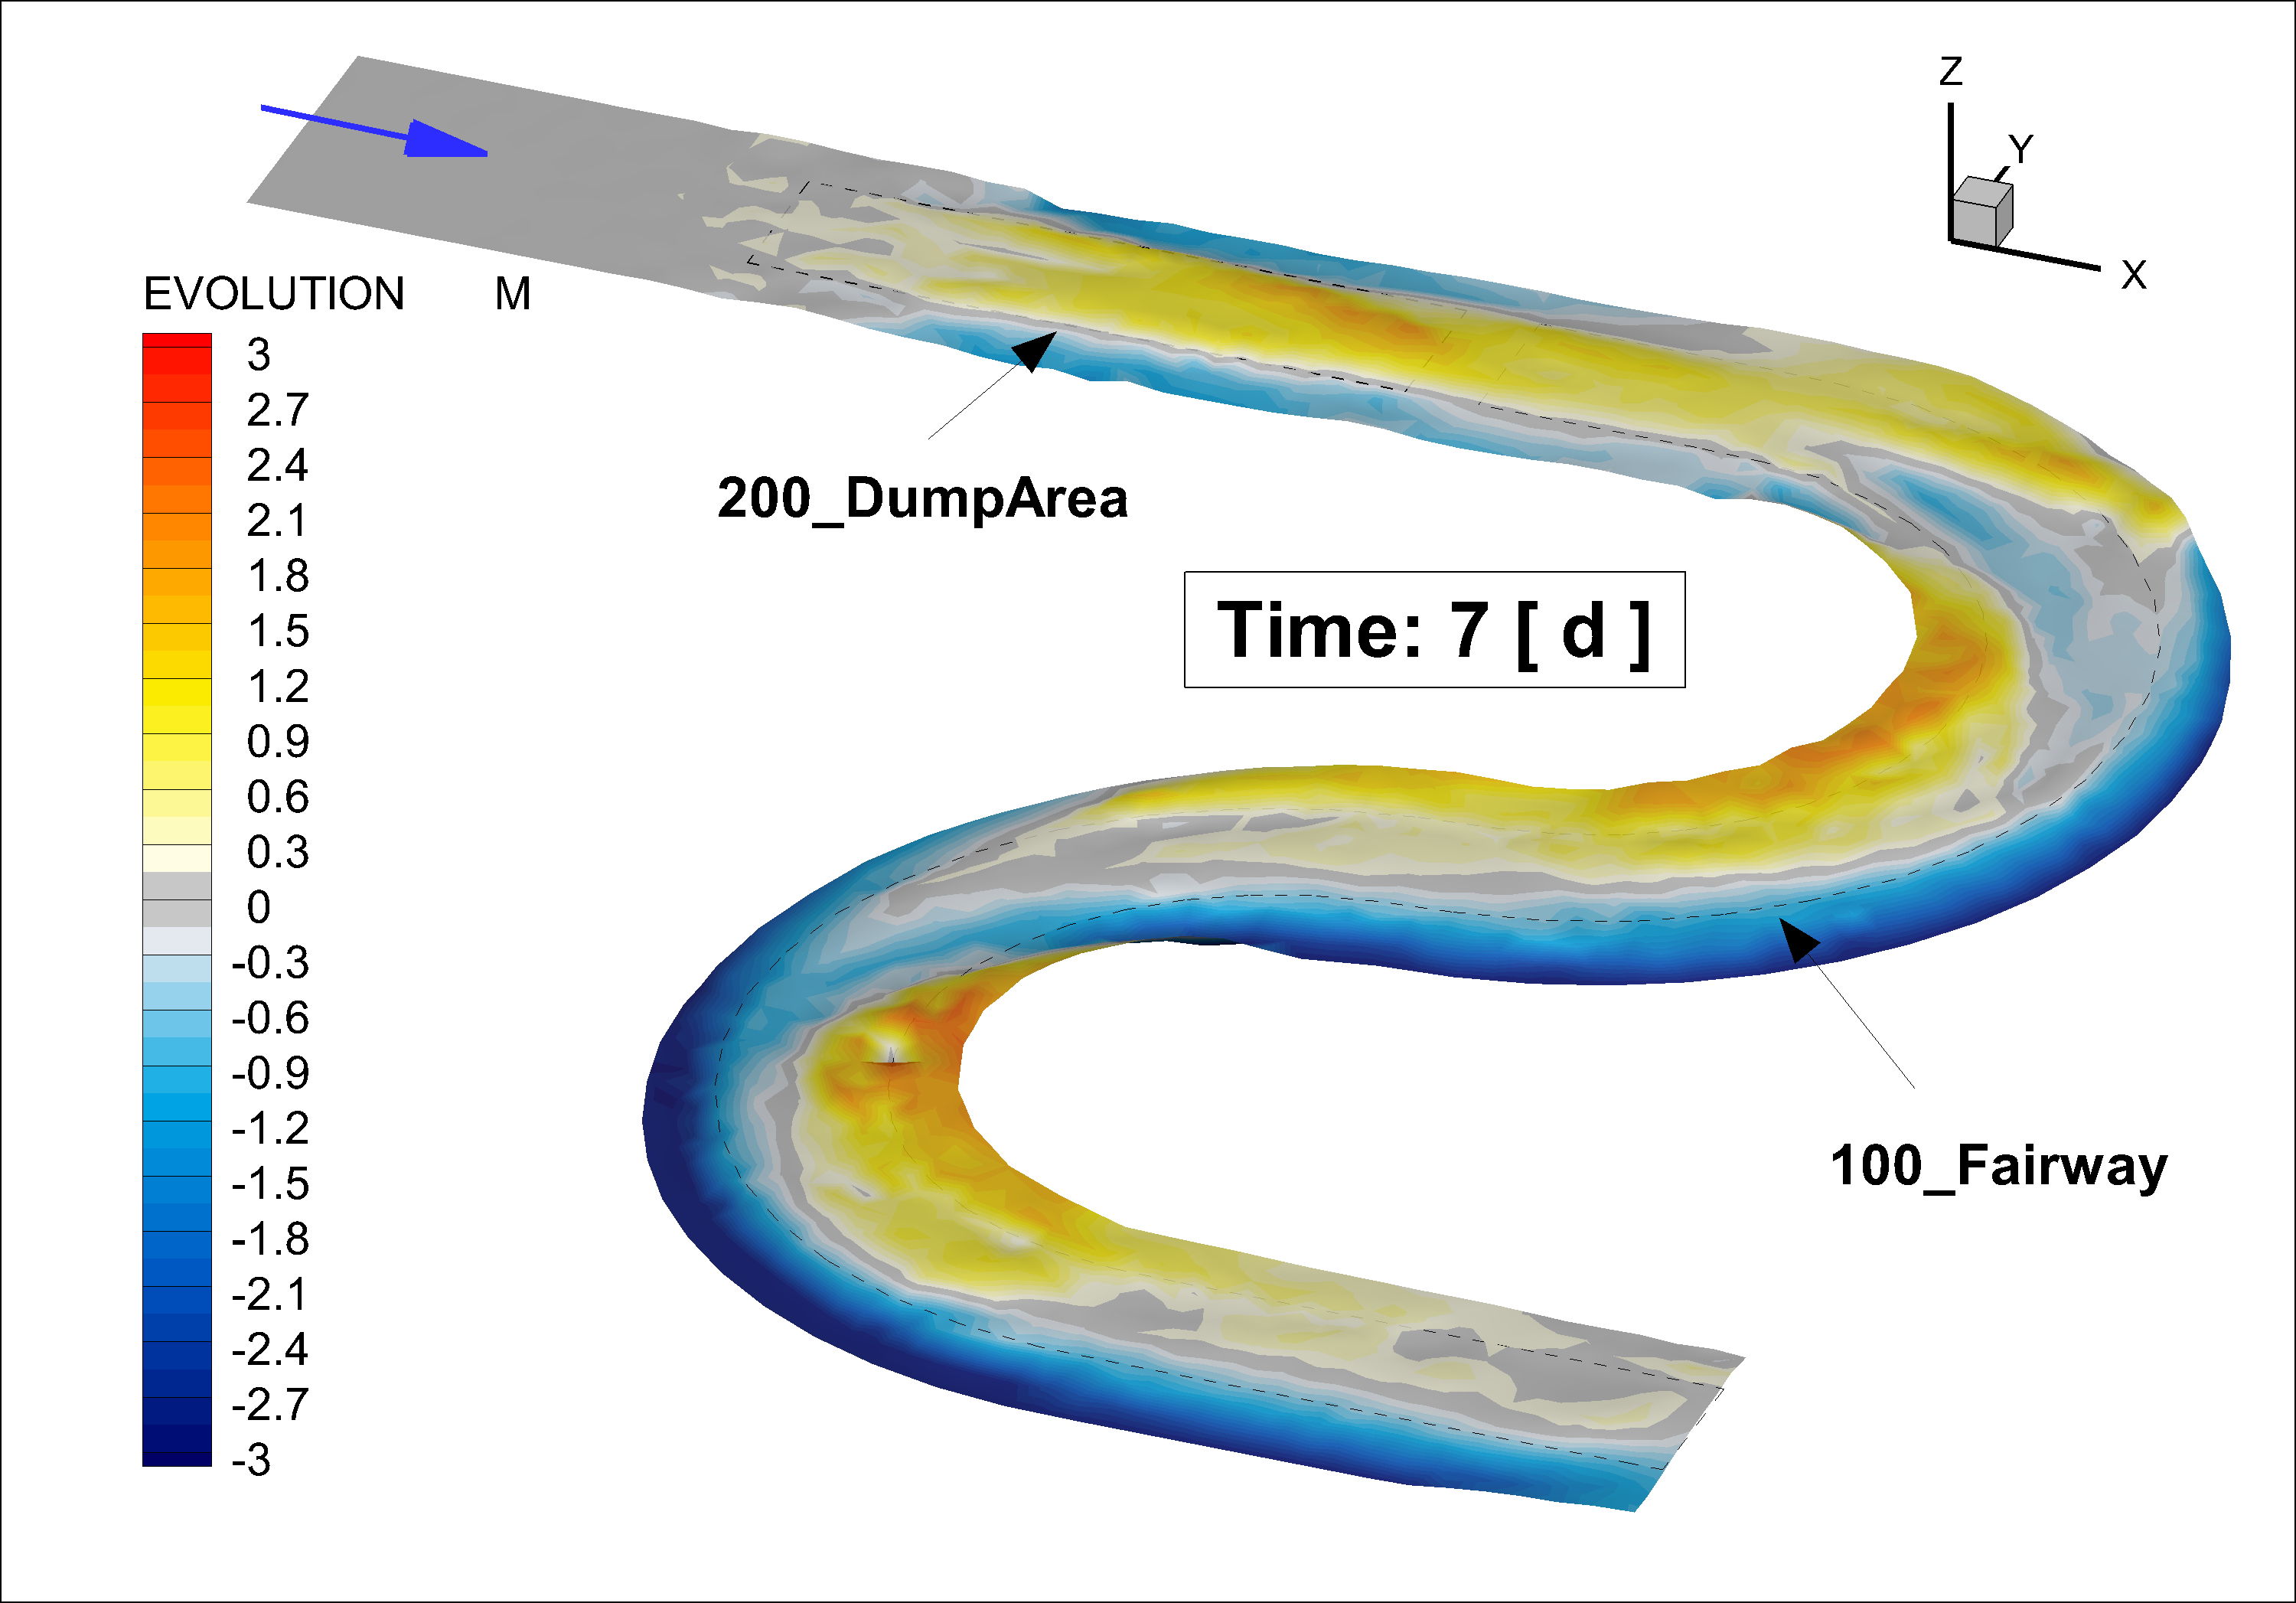
\includegraphics[scale=0.14]{img/critDig_Poly_07p0d.png}
\caption{Simulated evolution over the time.}\label{result34}
\end{figure}

\begin{figure} [!h]
\centering
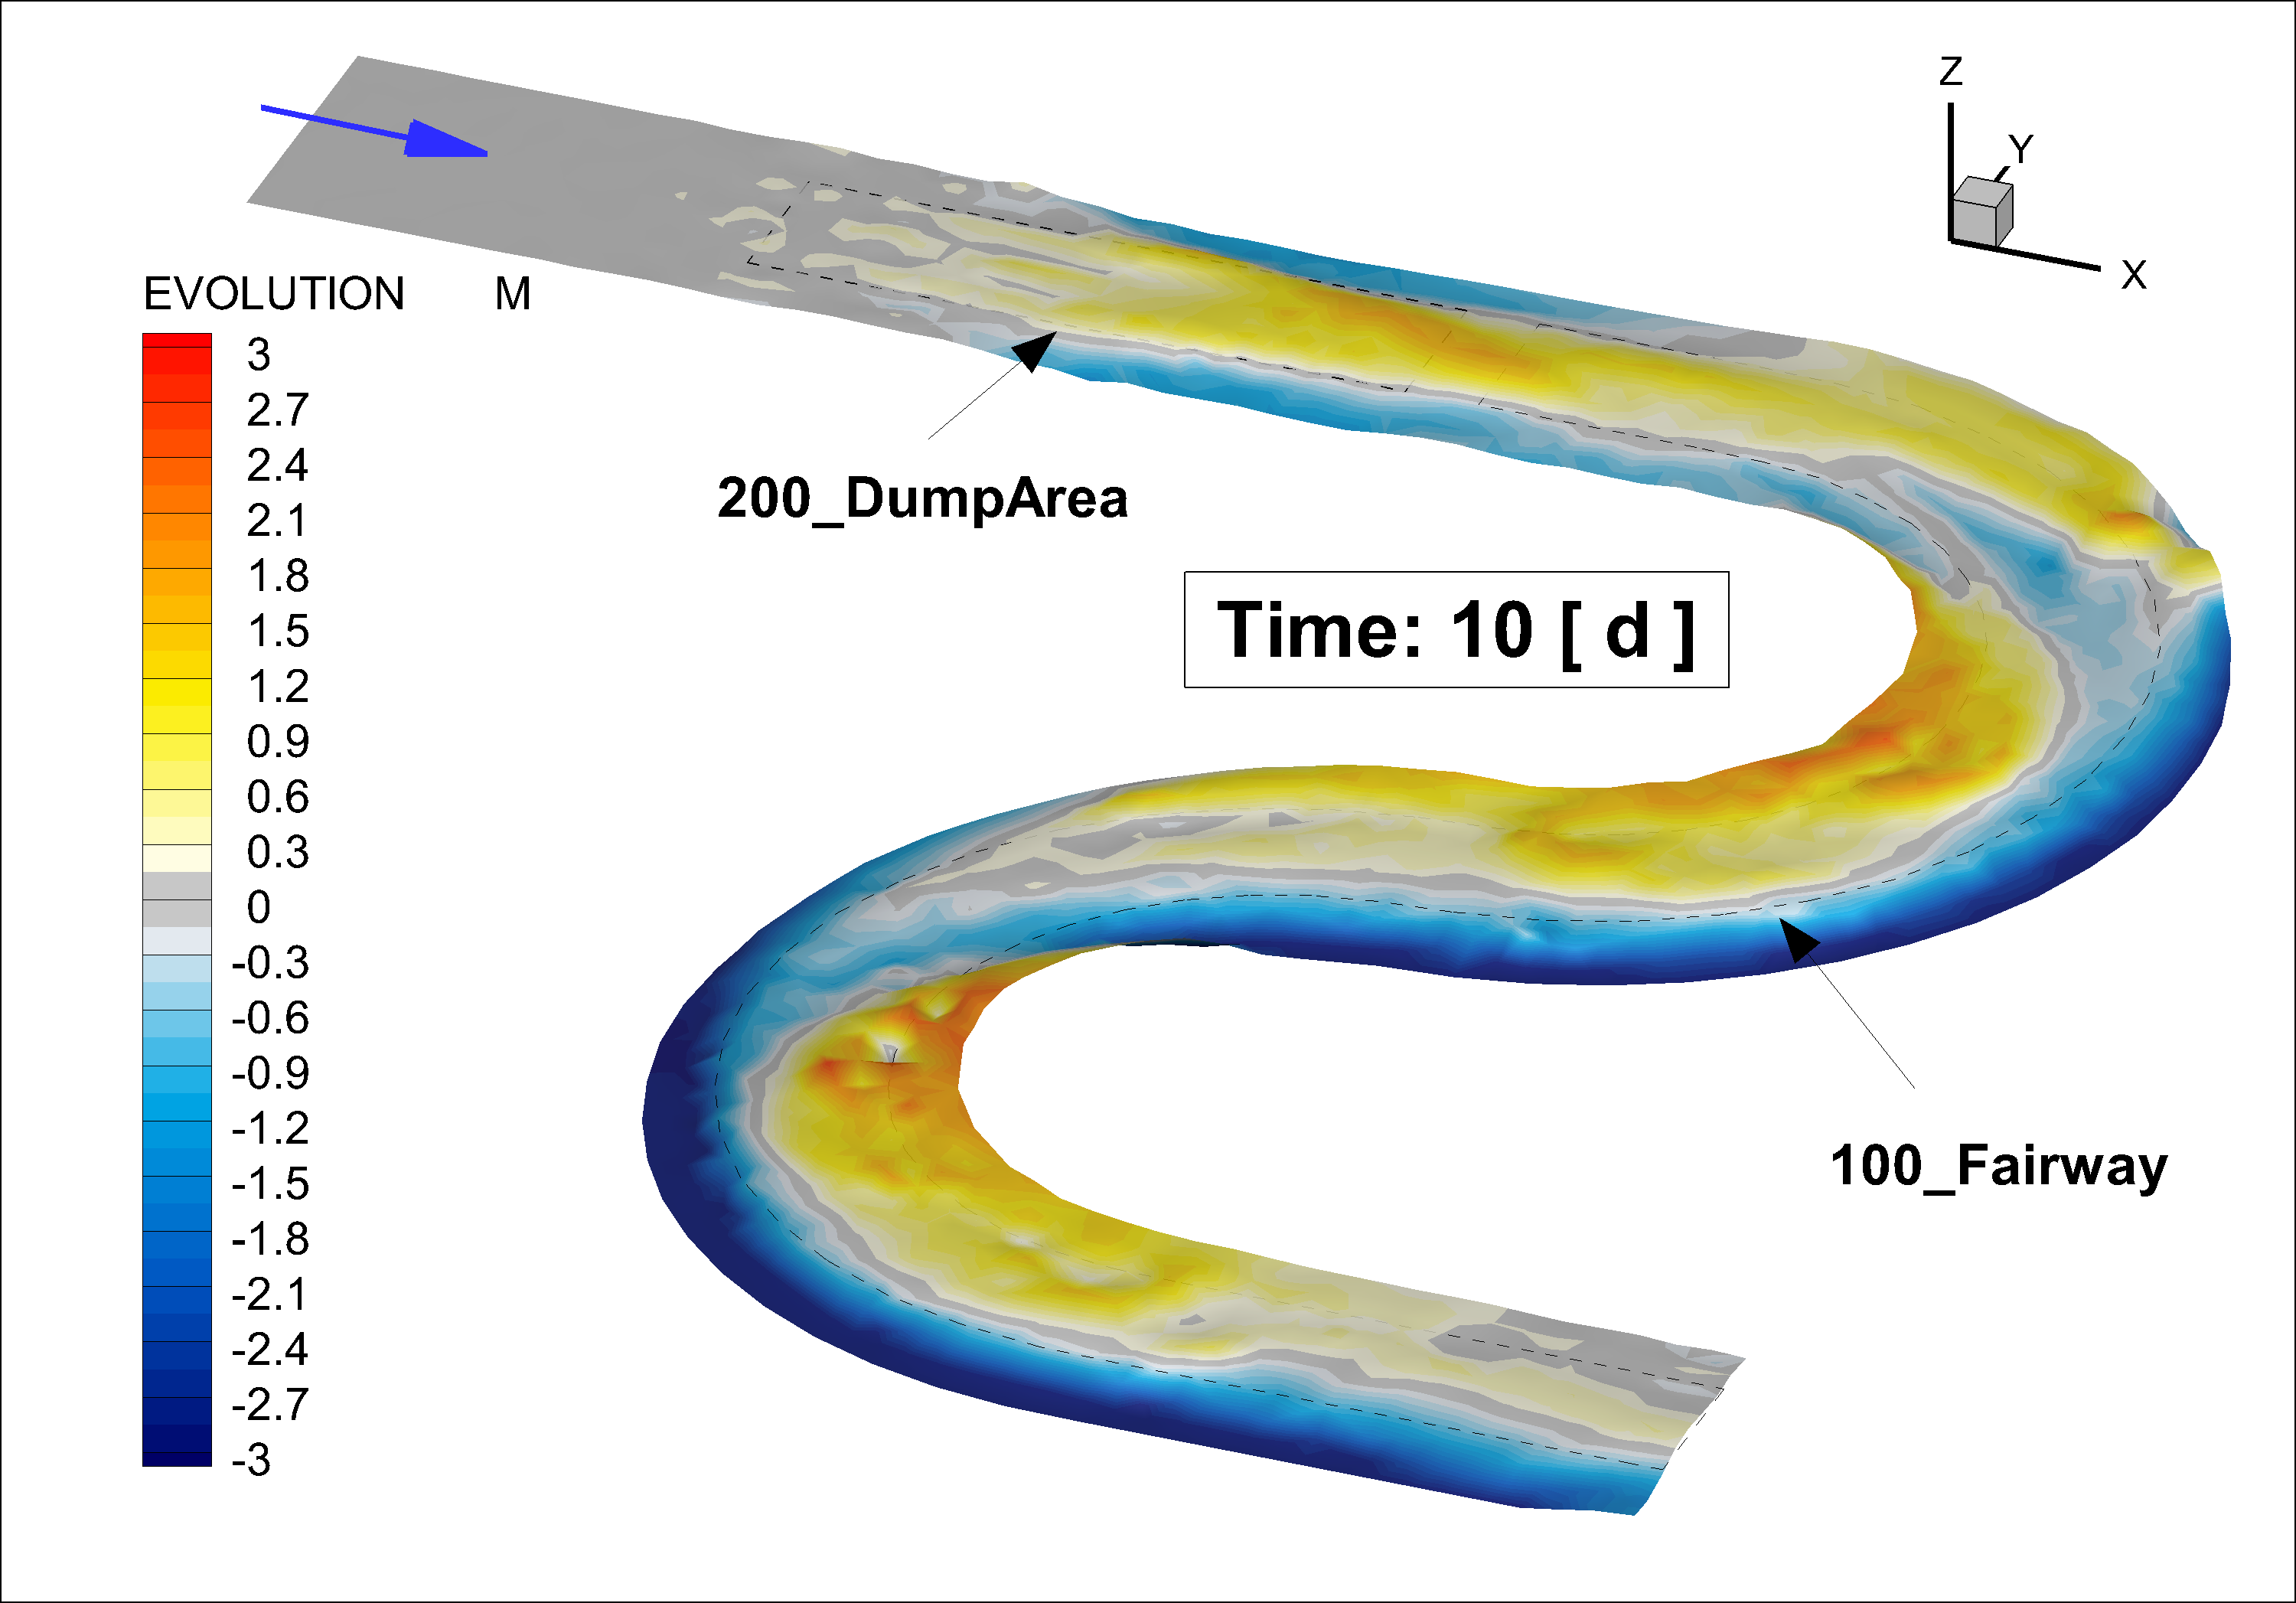
\includegraphics[scale=0.14]{img/critDig_Poly_10p0d.png}
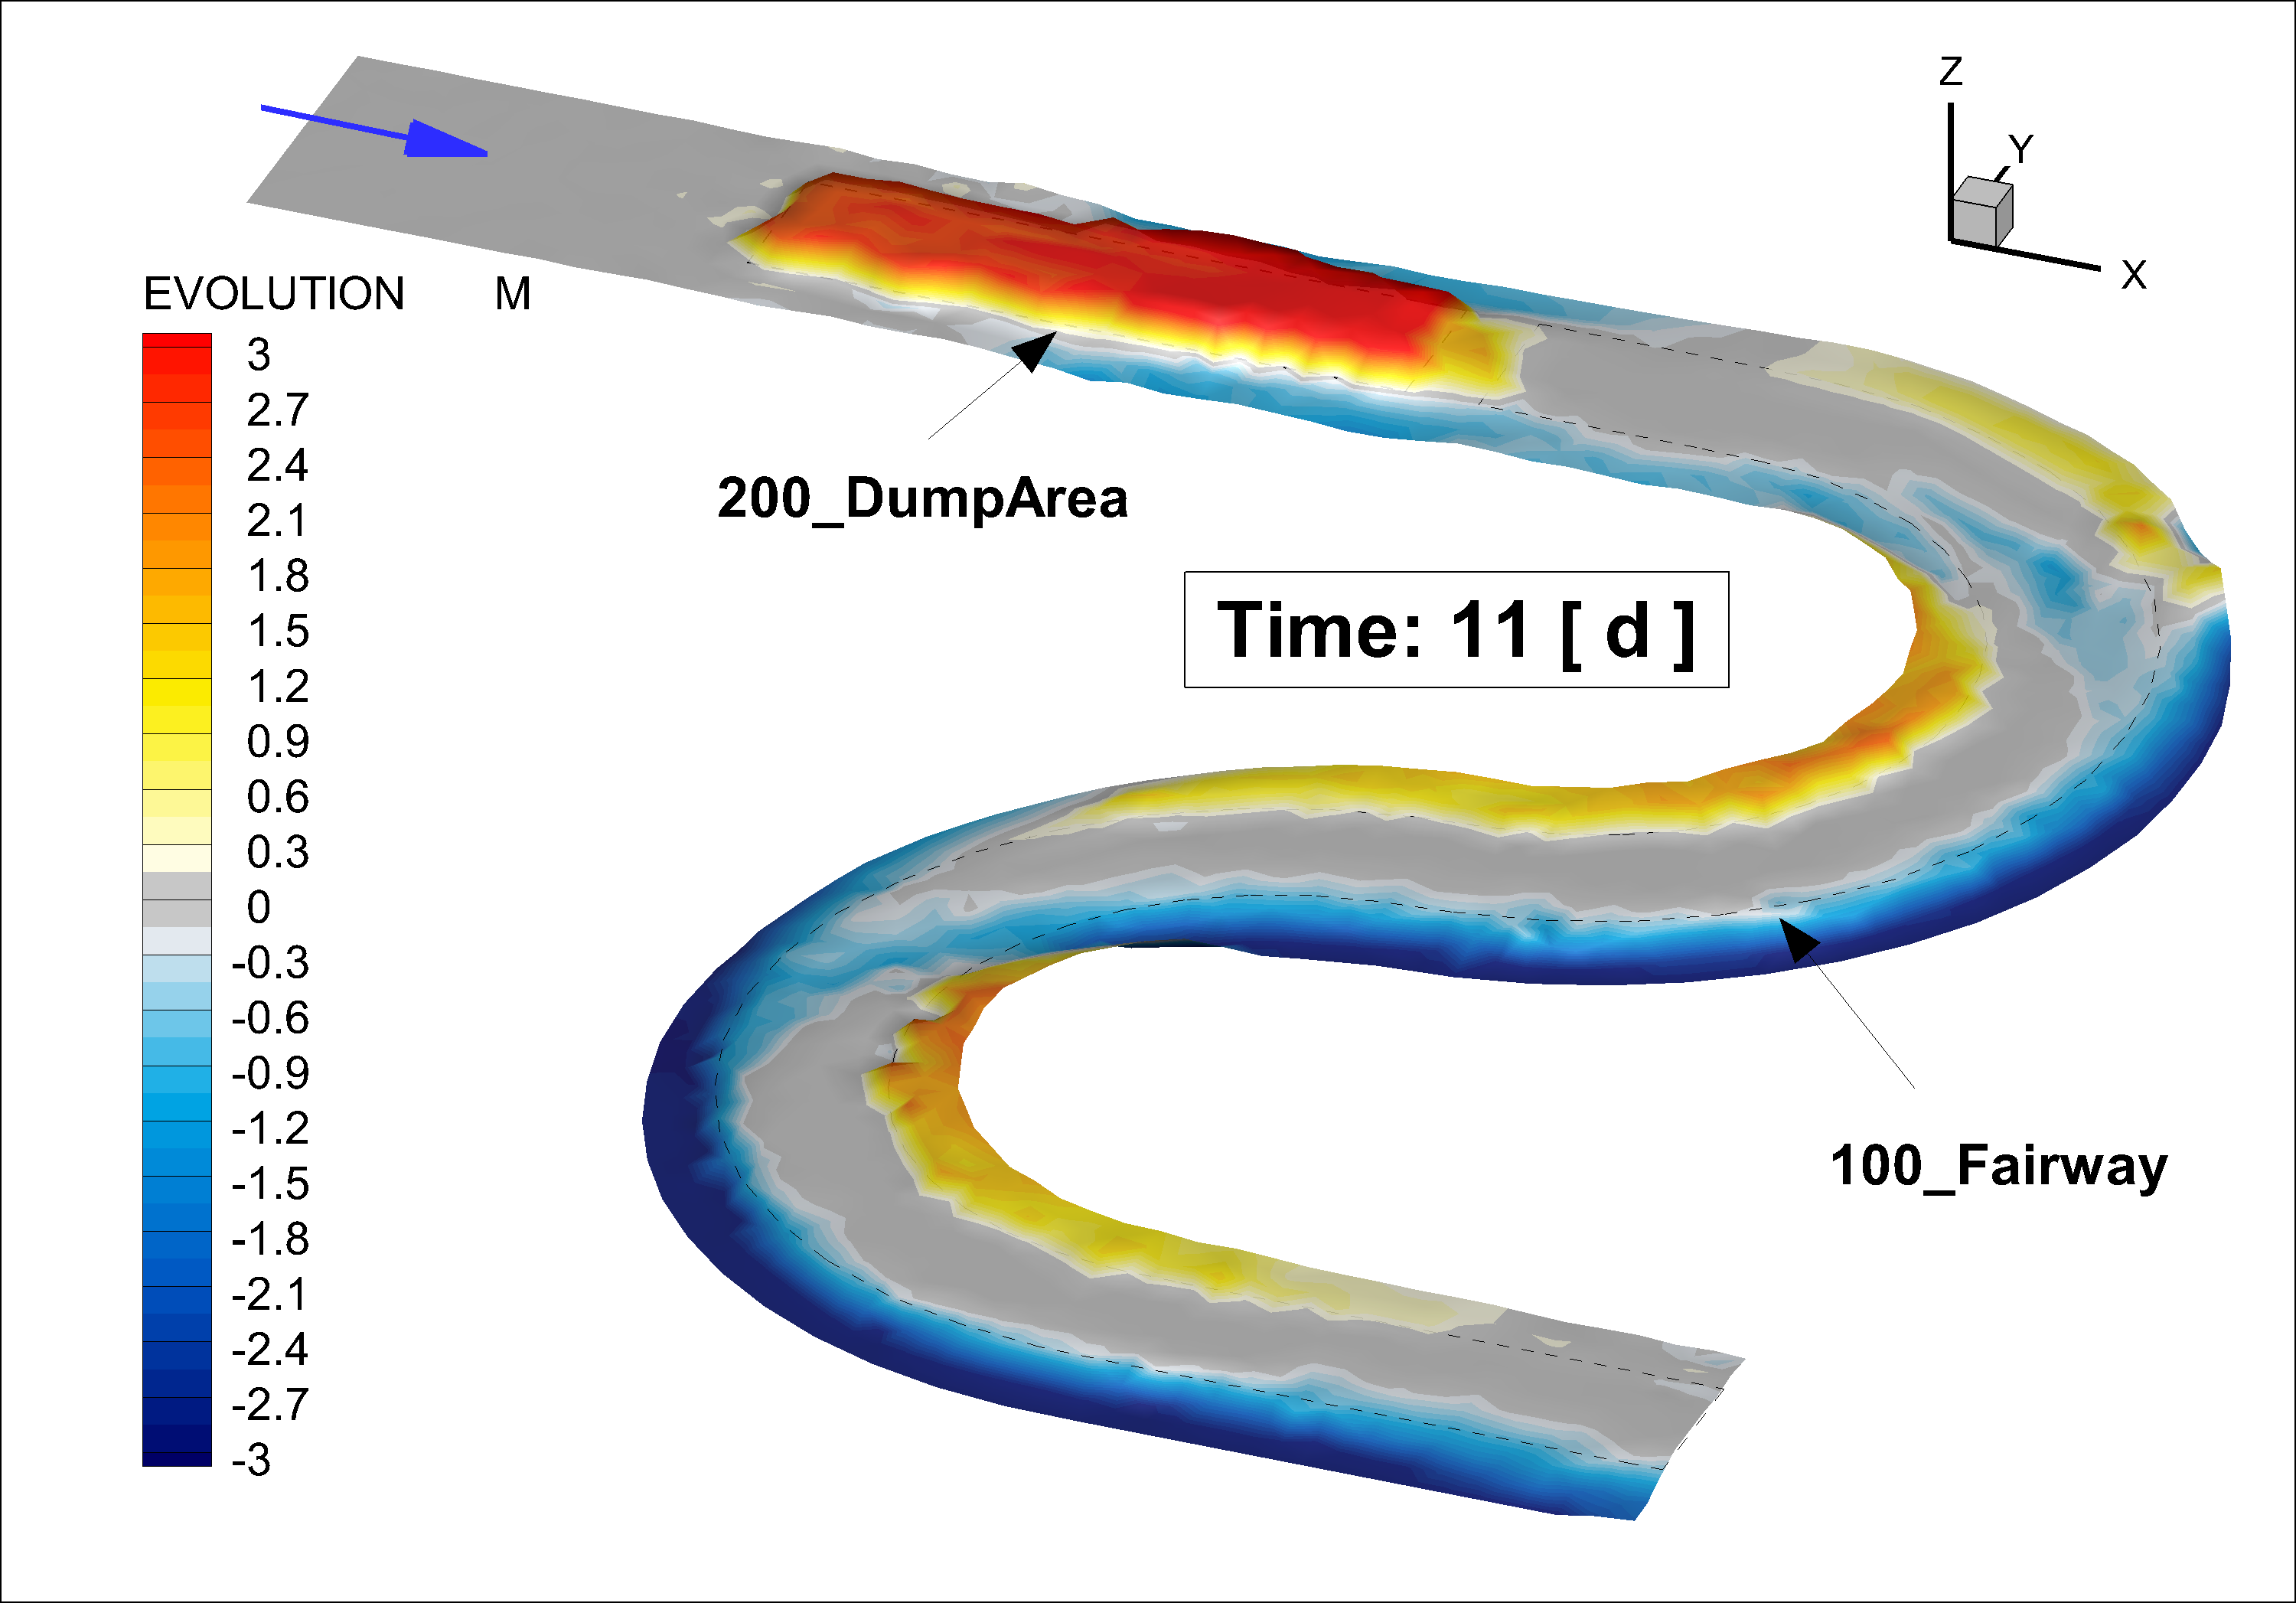
\includegraphics[scale=0.14]{img/critDig_Poly_11p0d.png}
\caption{Simulated evolution over the time.}\label{result56}
\end{figure}

\begin{figure} [!h]
\centering
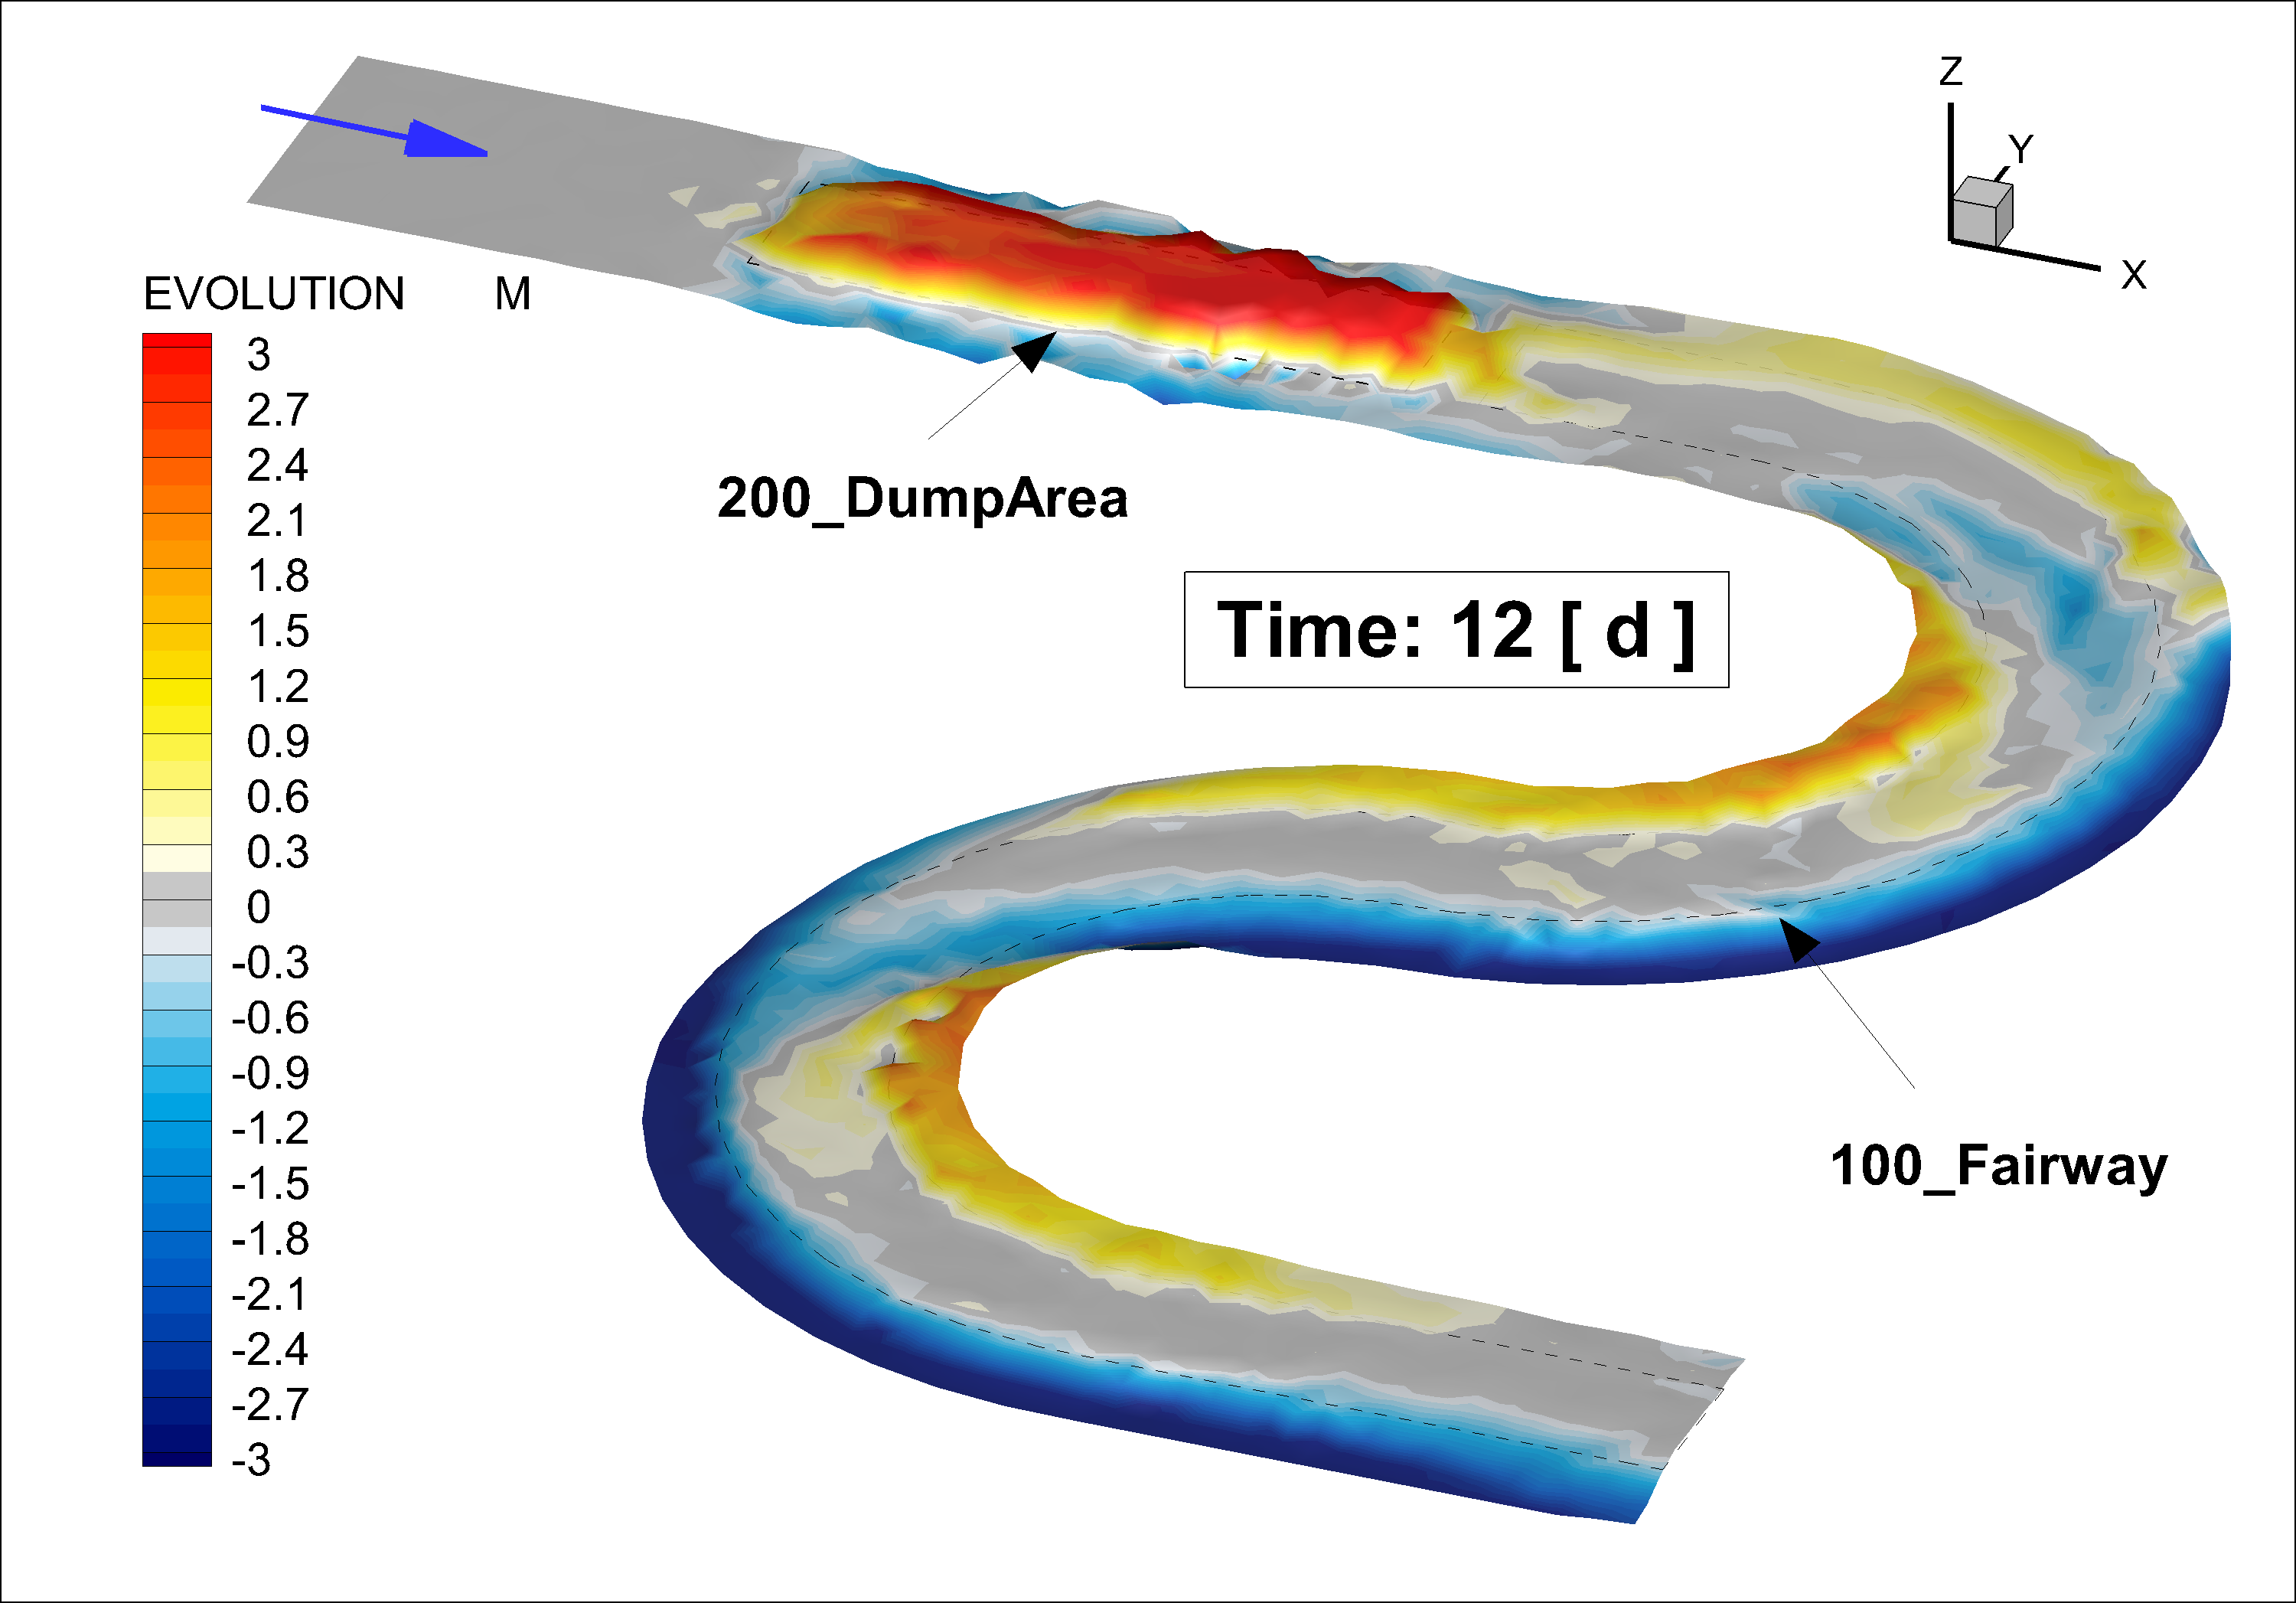
\includegraphics[scale=0.14]{img/critDig_Poly_12p0d.png}
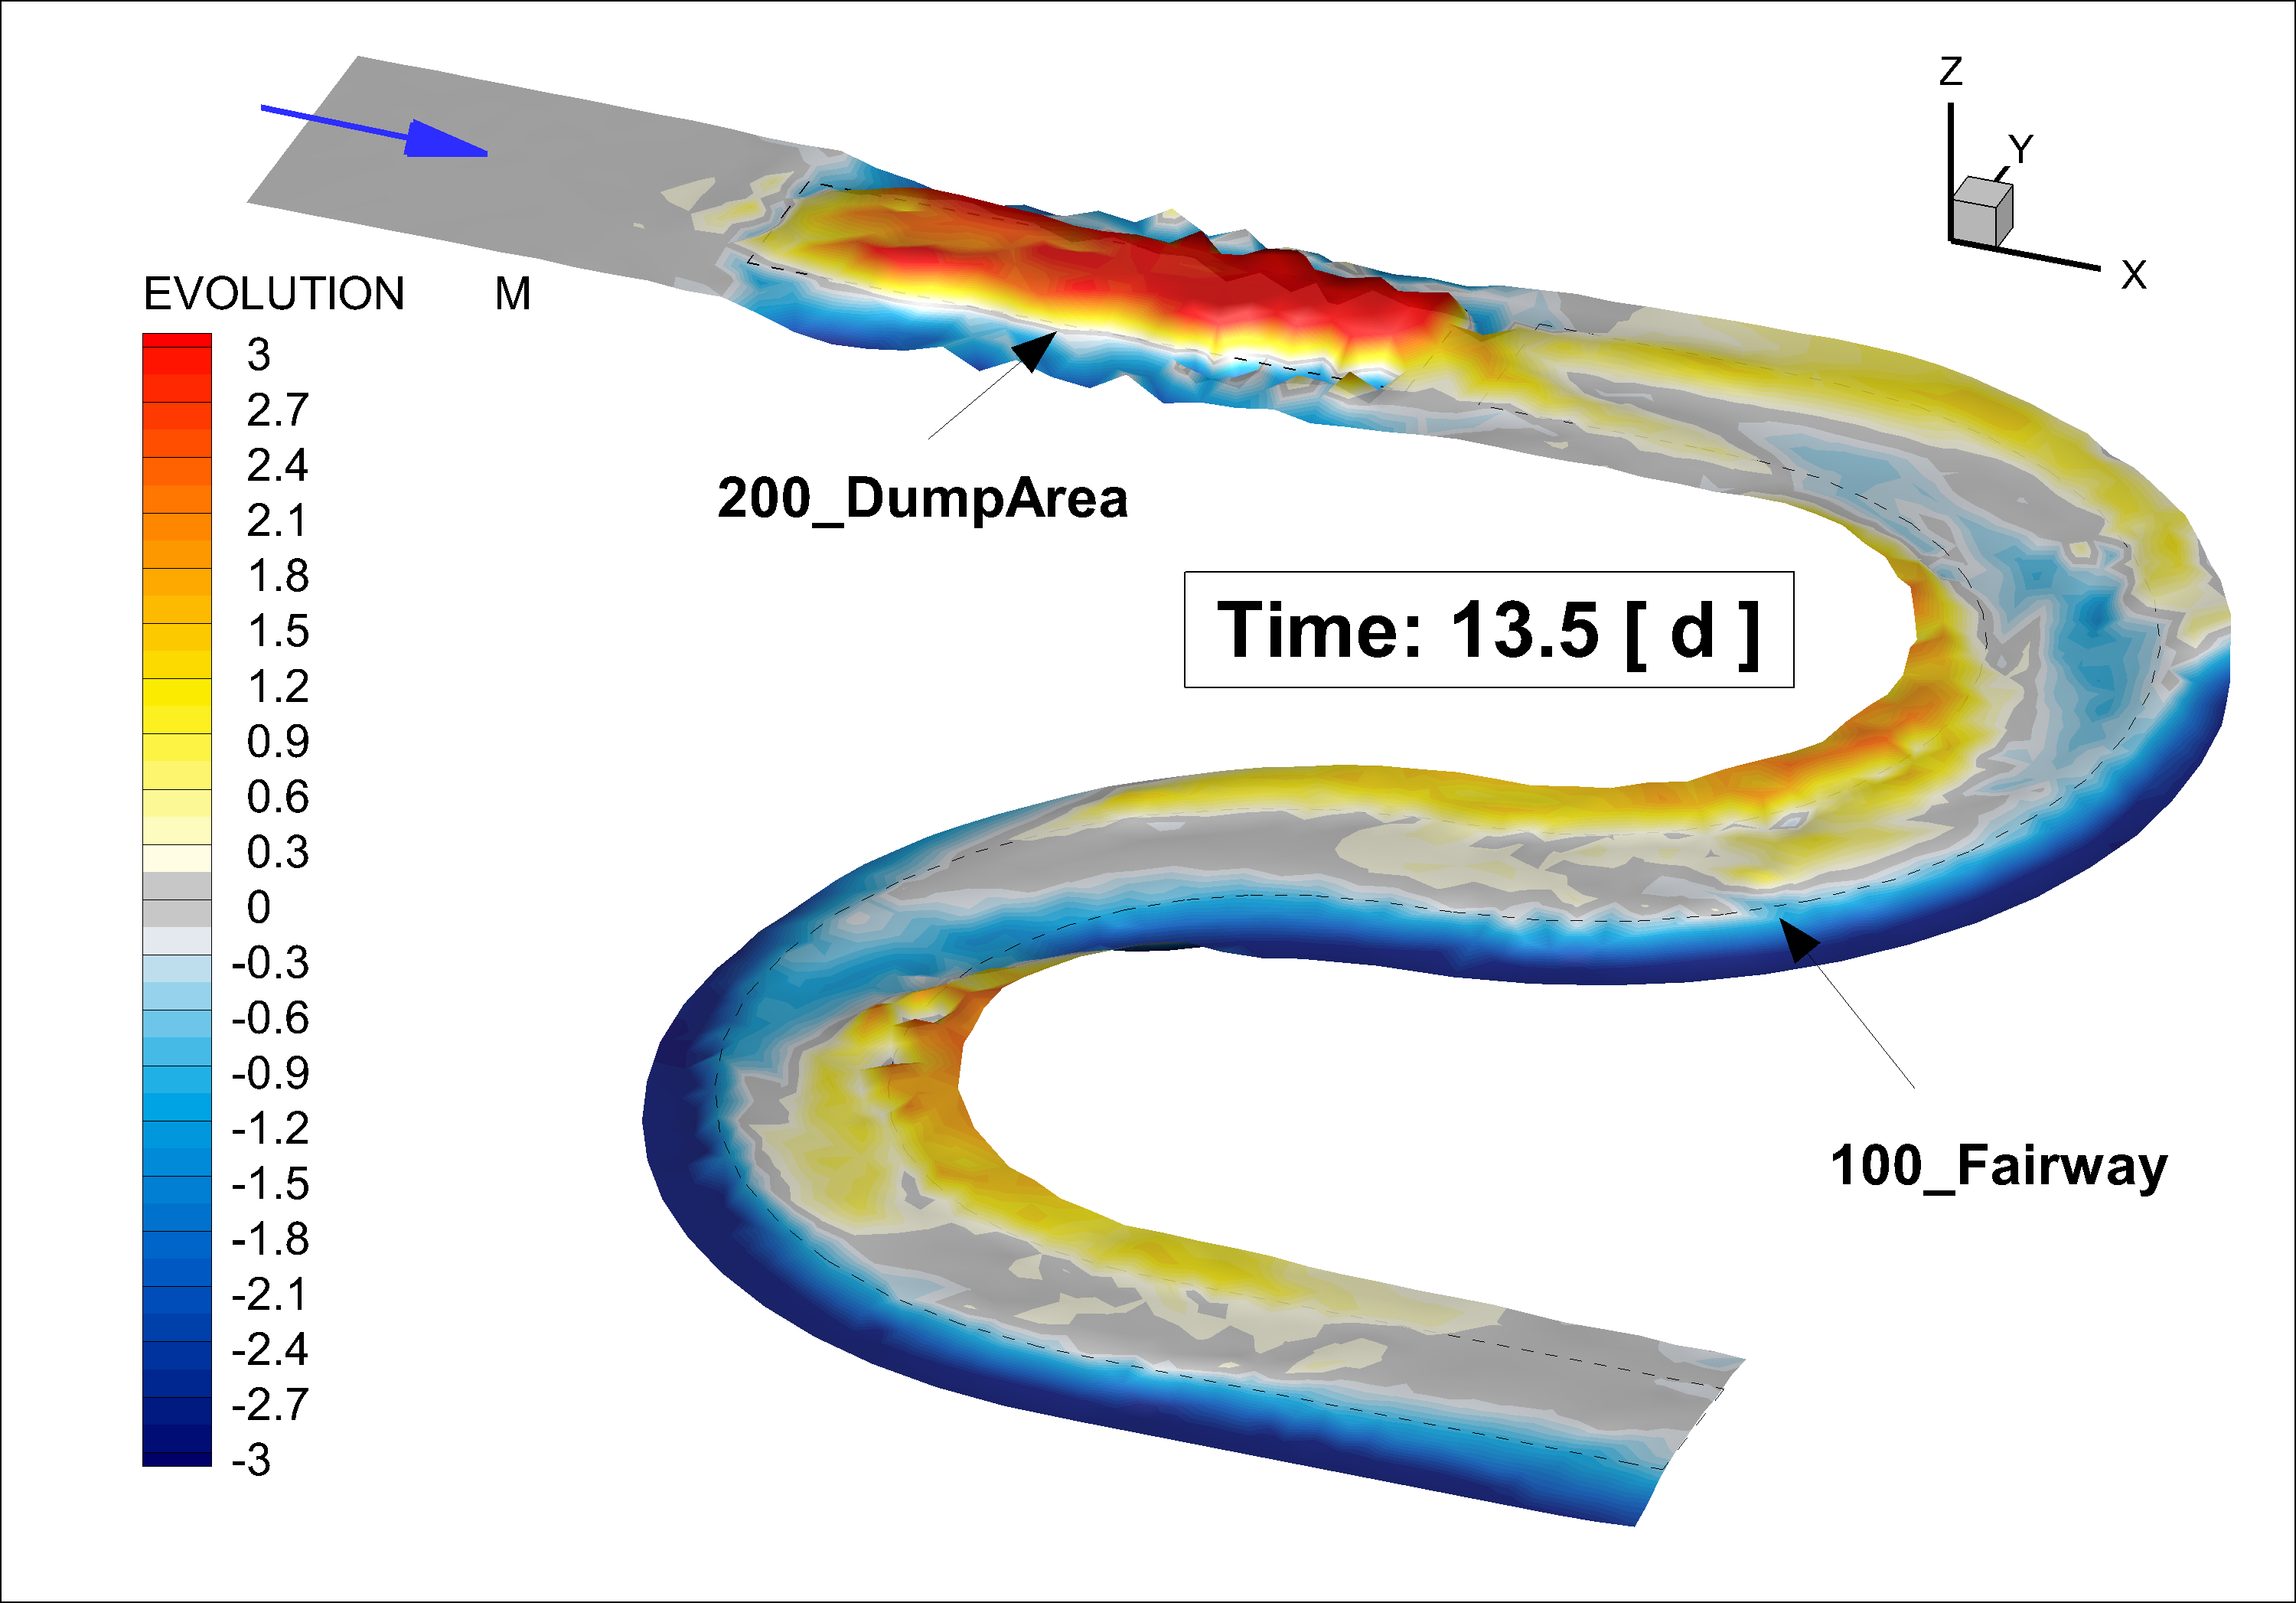
\includegraphics[scale=0.14]{img/critDig_Poly_13p5d.png}
\caption{Simulated evolution over the time.}\label{result78}
\end{figure}
